\documentclass[a4paper]{unicam_thesis}
\usepackage[sorting=none]{biblatex}
\usepackage[T1]{fontenc}
\usepackage[utf8]{inputenc}
\usepackage[italian]{babel}


%%%%%%%%%%%%%%%%%%%%%%%%%%%%
% TESI DATI FRONTESPIZIO
%%%%%%%%%%%%%%%%%%%%%%%%%%%%

\title{Brute Force \\ Wordlist, Bruteforce Strategies And CUDA }

\university{Universit\`a degli Studi di Camerino}%
\school{Scienze e Tecnologie}%
\course{Laurea in Informatica (Classe L-31)}%


\author{Nico Trionfetti}%
\advisor{Prof. Fausto Marcantoni}%
% \coadvisor2{Correlatore Name}%
\academicyear{2020/2021}%
\matricola{105381}%

%%%%%%%%%%%%%%%%%%%%%%%%%%%%
% FINE DATI FRONTESPIZIO
%%%%%%%%%%%%%%%%%%%%%%%%%%%%

\theoremstyle{definition} \newtheorem{esempio}{Esempio}[chapter]
\theoremstyle{definition}
\newtheorem{definizione}{Definizione}[chapter] \theoremstyle{plain}
\newtheorem{teorema}{Teorema}[chapter]
\graphicspath{{Screenshot/},{Immagini/},{API/},{Source/}}
\bibliography{biblio.bib}
\begin{document}

\maketitle


\tableofcontents

\abstract

I requisiti della \textbf{sicurezza informatica} all'interno delle organizzazioni e delle nostre nostre vite, hanno subito dei importanti cambiamenti nei ultimi anni. Prima della diffusione dei sistemi di elaborazione delle informazioni, la sicurezza delle informazioni era considerata principalmente un problema di carattere fisico e amministrativo. Per esempio, per conservare i documenti più importanti venivano utilizzati pesanti armadi con chiusura a combinazione.

Con l'introduzione dei computer e lo spostamento di questi documenti in formato digitale, divenne necessario utilizzare strumenti per la protezione di questi file e delle informazioni in essi memorizzate. Gli strumenti progettati per tenere sicuri questi dati, sono algoritmi di criptazione, che permettono di rendere inutilizzabile il dato, almeno che non si abbia la chiave per decifrarlo. Gli hacker però sono riusciti a trovare alcune tecniche che possono rendere invano il tentativo di proteggersi tramite l'utilizzo criptazione, queste tecniche utilizzate dai hacker prendono il nome di Brute Force. 

\addcontentsline{toc}{chapter}{Abstract}
\chapter{Introduzione}
\section{Che cos'è il Brute Force}
Nella crittografia , un attacco di Brute Force consiste in un utente malintenzionato che invia molte password con la speranza di indovinare una combinazione correttamente.

L'aggressore controlla sistematicamente tutte le possibili password finché non trova quella corretta. In alternativa, l'attaccante può tentare di indovinare la chiave che in genere viene creata dalla password utilizzando una funzione di derivazione della chiave.
\begin{figure}[h]
    \centering
    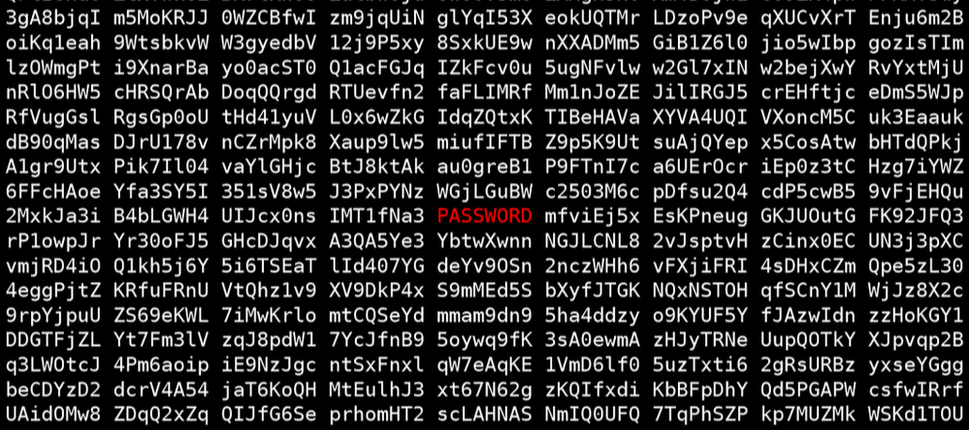
\includegraphics[width=115mm]{Immagini/introduzione/banner.png}
\end{figure}

Un attacco di Brute Force è un attacco crittoanalitico che, in teoria, può essere utilizzato per tentare di decrittografare qualsiasi dato crittografato. Tale attacco potrebbe essere utilizzato quando non è possibile sfruttare altri punti deboli in un sistema di crittografia che renderebbero il compito più semplice.

Gli attacchi di forza bruta funzionano calcolando ogni possibile combinazione che potrebbe costituire una password e testandola per vedere se è la password corretta. All'aumentare della lunghezza della password, la quantità di tempo e la potenza di calcolo richiesta in media per trovare la password corretta aumenta in modo esponenziale.

Per password più lunghe vengono utilizzati altri metodi come l' attacco del dizionario perché una ricerca a forza bruta richiede troppo tempo. Password e chiavi più lunghe hanno più valori possibili e persino più combinazioni, il che le rende esponenzialmente più difficili da decifrare rispetto a quelle più corte.

Gli attacchi di forza bruta possono essere resi meno efficaci offuscando i dati da codificare, rendendo più difficile per un utente malintenzionato riconoscere quando il codice è stato craccato o costringendo l'aggressore a fare più lavoro per testare ogni ipotesi. Una delle misure della forza di un sistema di crittografia è il tempo che teoricamente impiegherebbe un utente malintenzionato per sferrare un attacco di forza bruta riuscito contro di esso.
\section{Hash}
Le funzioni hash \cite{hash} sono particolari funzioni che permettono di dare a un messaggio un’impronta digitale tale da identificarlo univocamente.
\begin{figure}[h]
    \centering
    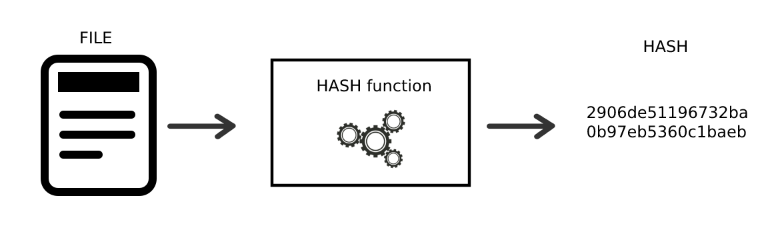
\includegraphics[width=115mm]{Immagini/introduzione/hash.png}
    \caption{hash}
    \label{fig:hash}
\end{figure}

In altre parole creano una stringa associata al messaggio da spedire e per il quale, una volta applicata la funzione, non dovrebbe essere più possibile ritornare al testo originale.
Quindi, il valore hash h(M) è una rappresentazione non ambigua e non falsificabile di un messaggio M, facile da calcolare e tale da comprimere il messaggio stesso.
Tra le principali proprietà delle funzioni hash ricordiamo che: sono facili da calcolare, godono della proprietà di sicurezza forte (è computazionalmente difficile trovare 2 messaggi diversi con lo stesso valore hash), godono della proprietà di sicurezza debole (dato M, è computazionalmente difficile trovare M’ tale che h(M) = h(M’)), e sono One-way, cioè, dato y è computazionalmente difficile trovare M tale che y = h(M).
\subsection{Types}
Le principali funzioni hash presenti attualmente sono:
\begin{itemize}
    \item \textbf{MD2}\newline  acronimo di Message Digest Algorithm, produce un valore hash di 128 bit e richiede come input multipli di 16 byte. La funzione, inoltre, usa un padding, cioè aggiunge dei bit mancanti ai messaggi in input che non hanno la lunghezza giusta. Questo algoritmo è già stato violato.
    \item \textbf{MD4}\newline anche questa funzione usa hash a 128 bit, ma è più veloce di MD2. Processa il messaggio dividendolo in blocchi di 512 bit. Il padding del messaggio, inoltre, comprende un valore di 64 bit che indica la lunghezza del messaggio originale. Questa funzione è più sicura della precedente, in quanto la difficoltà di produrre due messaggi che hanno la stessa lunghezza con modulo \(2^{64}\) è maggiore.
    \item \textbf{MD5}\newline è stato ideato dopo la violazione di MD4, su cui è basato. Il testo è diviso in blocchi 512 bit e viene generato un hash di 128 bit. E’ basato su XOR e operazioni logiche. L’unico svantaggio è dovuto dal fatto che è un po’ più lento di MD4.
    \item \textbf{SHA-1}\newline  acronimo di Secure Hash Algorithm-1 (anche SHS, Secure Hash Standard), sviluppato dal NSA su richiesta del NIST (National Institute of Standard and Technology). Utilizza gli stessi principi di MD4 e MD5. Il progetto originale del 1994 aveva il nome di SHA, poi modificato nel codice dal NSA. Produce output di 160 bit a partire da una lunghezza arbitraria. Attualmente è uno dei più sicuri, usato anche dai servizi PGP e GPG per firmare documenti.
    \item \textbf{SHA-2}\newline versione successiva a SHA-1, genera impronte di documenti da 256, 384 e 512 bit.
\end{itemize}
\section{Password analysis}
Una cosa da conoscere per effettuare un buon attacco di Brute Force, è la composizione di una password e la sua tassonomia \cite{hashcrack}, da uno studio generale delle password è stato notato che :
\begin{itemize}
    \item la lunghezza media di una password è di 7 - 9 caratteri
    \item si ha il 50\% di possibilità che una password contenga una o più vocali
    \item le donne preferiscono utilizzare nomi per le loro password e gli uomini preferiscono gli hobby
    \item i simboli più utilizzati sono : \textasciitilde, !, @, \#, \$, \%, \&, *, e ?
    \item se si utilizza un numero è il 1 o il 2 e sono utilizzati alla fine
    \item se si utilizza più di un numero, sono sequenze o numeri personali
    \item se si utilizza una lettere maiuscola, questa si trova all'inizio
    \item 66\% delle persone utilizza 1-3 password per tutti i suoi account
    \item una persona su nove ha una password basata sulle 500 password più utilizzate
    \item i paesi occidentali preferiscono le password in minuscolo e i paesi dell'est preferiscono le cifre
\end{itemize}

Le password possono contenere molte informazioni al riguardo al suo creatore, molte volte la stessa persona utilizza un pattern specifico per la creazione delle proprie password, dove andrà a cambiare piccoli dettagli tra una password e l'altra.
Questi pattern si possono suddividere in :
\begin{itemize}
    \item \textbf{Basic Pattern}\newline
          Visibile facilmente, composto da gruppi ben distinti\newline
          \begin{figure}[h]
              \centering
              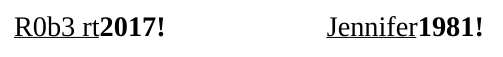
\includegraphics[width=\linewidth]{Immagini/introduzione/Basic_Pattern.png}
              \caption{Basic Pattern}
              \label{fig:basic}
          \end{figure}
          \newline Qui possiamo notare che ogni password è composta da un nome e termina con quattro numeri con lo stesso carattere speciale \!.
    \item \textbf{Macro Pattern}\newline
          Statiche sulla struttura come lunghezza e set di caratteri\newline
          \begin{figure}[h]
              \centering
              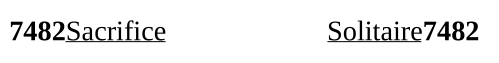
\includegraphics[width=\linewidth]{Immagini/introduzione/Macro_pattern.png}
              \caption{Macro Pattern}
              \label{fig:macro}
          \end{figure}
          \newline Qui possiamo notare che le password hanno un loro schema, composto dalla combinazione di 4 numeri e 7 lettere, inoltre la parola inizia in entrambi i casi con una maiuscola ed in entrambi i casi abbiamo sempre la stessa lettere e lo stesso gruppo di numeri.
    \item \textbf{Micro Pattern}\newline
          Utilizzo di temi e dati/interesse personali per la loro composizione\newline
          \begin{figure}[h]
              \centering
              \includegraphics[width=\linewidth]{Immagini/introduzione/Micro_Pattern.png}
              \caption{Micro Pattern}
              \label{fig:micro}
          \end{figure}
          \newline Qui possiamo notare che ogni password inizia con un colore, inoltre la seconda parte è composta da un nome di un animale e si utilizzano 3 numeri diversi per concludere la password.
\end{itemize}

L'individuazione di queste schemi possono andare a ridurre di molto i tempi che si impiegano per trovare le password, perché ci permettono di capire quale tecnica è più adeguata da applicare e quali regole applicare per l’esecuzione dell’attacco.

\subsection{20-60-20 RULE}

La regola 20-60-20 è un modo per visualizzare il livello di distribuzione delle password in base alla loro complessità, con caratteristiche che generalmente seguono quelle di una curva gaussiana, dove sull'asse delle X abbiamo la complessità della password e sul lato delle Y abbiamo il "numero" di quante persone la utilizzano.
\begin{itemize}
    \item Il 20\% delle password sono parole del dizionario facilmente indovinabili o password comuni.
    \item Il 60\% delle password sono variazioni da moderate a leggere rispetto al precedente 20\%.
    \item Il 20\% delle password sono rigide, lunghe, complesse o con caratteristiche uniche.
\end{itemize}

\begin{figure}[htpb!]
    \centering
    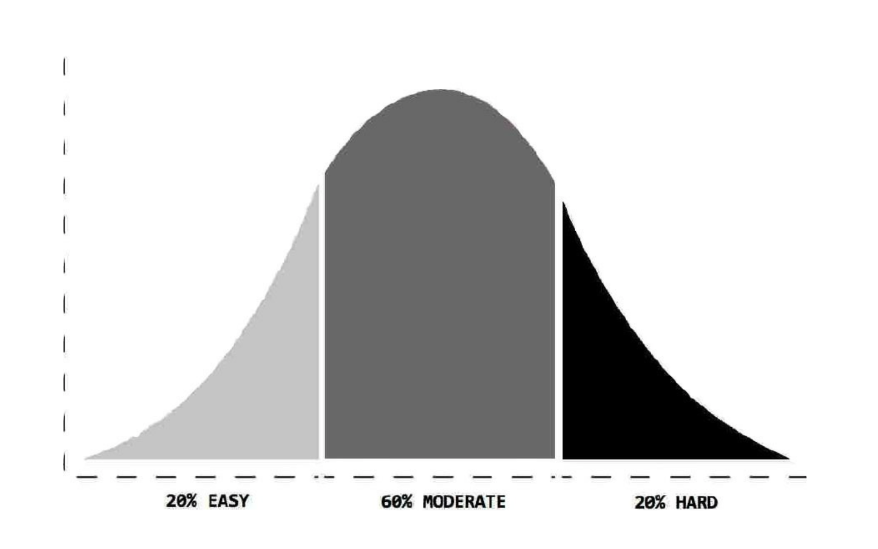
\includegraphics[width=\linewidth]{Immagini/introduzione/20-60-20.png}
    \caption{Rule 20-60-20 \cite{hashcrack}}
    \label{fig:rocker}
\end{figure}



\chapter{Tecniche di Brute Force}
Quando un hacker utilizza la forza bruta per sferrare un attacco brute force, solitamente lo fa per risalire a una password, a un PIN o a una chiave crittografica.

In pratica, l'hacker tenta di accedere a un account o a dei file protetti utilizzando un metodo automatizzato che procede per tentativi fino ad ottenere l'accesso desiderato.

Questo metodo, chiamato in inglese trial-and-error (tentativo ed errore), non richiede l'uso di algoritmi complessi ma semplicemente di tempo e potenza di calcolo.

L'attacco forza bruta è, sostanzialmente, l'equivalente di provare tutte le chiavi presenti nel proprio portachiavi fino a trovare quella giusta per aprire la porta di casa.

In ambito informatico, la serratura è l'account o il file a cui si vuole accedere, mentre le chiavi sono tutte le password possibili.

Ovviamente, tali password sono moltissime e quindi sarebbe impossibile procedere per tentativi manualmente, ma programmi appositi sono in grado di eseguire numerosi tentativi in intervalli di tempo molto brevi.

Per eseguire un attacco di forza bruta si può ricorrere a diversi metodi, che possono essere riconducibili alle tipologie elencate di seguito.
\section{Offline Attack}

Un utente malintenzionato può ottenere un hash della tua password che può portare offline \cite{Offline_attack} e provare a decifrarlo.

Un hash è solo una forma di crittografia unidirezionale. Quando il tuo computer salva la tua password, non salva (o non dovrebbe) salvarla in chiaro. Invece, esegue l'hashing della tua password e la salva. Quindi, ad esempio, se la tua password è Password123, il tuo computer memorizzerà: 42f749ade7f9e195bf475f37a44cafcb. In questo modo, se qualcuno è in grado di leggere la memoria del tuo computer, non sarà in grado di sapere qual è la tua password.

Ora, quando accedi al tuo computer, il computer prende ciò che hai inserito nella richiesta della password, calcola un hash e confronta quell'hash con quello che ha memorizzato quando hai impostato la password. Se le password corrispondono, ti viene concesso l'accesso. Un attacco con password offline porterà questo hash offline e cercherà di trovare il valore di testo non crittografato che calcola su quell'hash. Per fare ciò, un utente malintenzionato utilizza un computer per prendere le password, calcola l'hash e lo confronterà molto rapidamente. Questa operazione verrà eseguita più e più volte fino a quando non verrà trovata una corrispondenza.

La differenza tra attacchi di password offline e online è enorme. In un attacco con password offline, l'autore dell'attacco non tenta mai di accedere al server delle applicazioni. Ciò significa che è invisibile al team di sicurezza e ai log. Ciò significa anche che le protezioni comuni come i blocchi degli account non funzioneranno. Questo perché l'attaccante lo porterà offline, troverà la password e quindi solo un tentativo corretto verrà registrato dall'applicazione.

Un'altra importante differenza tra gli attacchi di password offline e online è la velocità. Mentre gli attacchi con password online sono limitati dalla velocità della rete, gli attacchi con password offline sono limitati solo dalla velocità del computer che l'aggressore sta utilizzando per violarli. Per contestualizzare, abbiamo una macchina di cracking che può tentare 3 miliardi di tentativi di password al secondo. Ciò significa che una password di 8 caratteri può essere brutalmente forzata (ogni possibile combinazione di caratteri) in meno di 3 giorni.

Parte fondamentale del Brute Force è l'utilizzo di strumenti adeguati in base all'operazione da svolgere.
Esistono molti programmi per recuperare le password dai Hash, i più famosi per l'utilizzo offline sono :
\begin{itemize}
    \item \textbf{HASHCAT}\cite{hashcat}
    \item \textbf{JOHN THE RIPPER}\cite{John_The_Ripper}
\end{itemize}
Questi consentono di decifrare una password andando a utilizzare diverse tecniche di Brute Force, con versatilità e velocità.
Inoltre hanno il supporto alla maggior parte dei tipi di criptazione e sono in grado sia di utilizzare la potenza computazionale della CPU e della GPU.

\section{Brute Force Attack}
Un attacco di forza bruta \cite{Brute_attack}\cite{Brute_attack2} è un tentativo di decifrare una password o un nome utente oppure di trovare una pagina web nascosta o la chiave utilizzata per crittografare un messaggio utilizzando l'approccio della prova e dell'errore con la speranza, alla fine, di indovinare. Si tratta di un vecchio metodo di attacco, ma è ancora efficace e molto usato dagli hacker.
A seconda della lunghezza e complessità della password, la sua individuazione può richiedere da pochi secondi a molti anni.

\begin{table}[h]
    \centering
    \begin{tabular}{ |c|c|c|c| }
        \hline
        Key Lenght (Chars) & Time To Decrypt \\
        \hline
        8                  & 15 min          \\
        \hline
        9                  & 14 hours        \\
        \hline
        10                 & 457 hours       \\
        \hline
        11                 & 3.3 years       \\
        \hline
        12                 & 214 years       \\
        \hline
    \end{tabular}
    \label{fig:brute}
    \caption{Tempo di Brute-Force (Password che comprende 0-9,a-z,A-Z)\cite{hashcrack}}
\end{table}

\section{Dictionary Attack}
Questo tipo di attacco \cite{Dictionary_attack} è forse quello più usato nell’ambito del Password Cracking. Perché permette di ottenere buoni risultati se il dizionario usato è completo e se le regole (rules) sono efficaci.

Il funzionamento è semplice, l’algoritmo segue questi step:
\begin{itemize}
    \item \textbf{Step 1}\newline Si prende la password in chiaro dal Dizionario e si genera l’hash (encrypt).
    \item \textbf{Step 2}\newline Si compara l’hash generato con l’hash della password da craccare.
    \item \textbf{Step 3}\newline Nel caso in cui l’hash non corrisponda, ritorna allo Step 1. \newline Nel caso in cui l’hash corrisponda, la password è stata trovata.
\end{itemize}

Proteggersi da questo attacco è semplice. Basta scegliere delle password non troppo convenzionali e banali.

Il successo di un attacco dipende largamente dal dizionario utilizzato, ma anche dal tipo di rules che applichiamo ad ogni voce del dizionario. Le “regole“, in generale, permettono di generare più varianti di una singola voce nel dizionario. Ad esempio, una possibile regola potrebbe essere denotata con "\textbf{-pl}" ad indicare al nostro software di cracking di effettuare e testare anche il plurale di ogni voce nel dizionario. Oppure "\textbf{[0-9]}" ad indicare di testare per ogni voce nel dizionario anche la variante che prevede un numero da 0 a 9 posto alla fine della stringa. I software di password cracking che permettono attacchi dizionario quasi sempre prevedono la possibilità di applicare regole. E’ anche importante saper configurare il nostro software per sfruttare le caratteristiche comuni e statisticamente più usate nella scelta di una password.

Nella rete possiamo trovare molti dizionari, ormai diventati standard grazie allora loro vasta scelta di password contenute e alla loro suddivisione per tipo ( password account / wi-fi / ecc ecc ), uno dei più utilizzati è \textbf{rockyou}, che contiene 14,341,564 password uniche , usate in 32,603,388 account.

Inoltre grazie a diversi strumenti possiamo generare dei dizionari personalizzati, in base ad esempio ad alcune informazioni che abbiamo recuperato sulla vittima del nostro attacco, lo strumento che ci permette di fare questo è \textbf{CRUNCH}\cite{CRUNCH}, che attraverso il seguente comando permette la creazioni di elenchi di parole in cui è possibile specificare un set di caratteri standard o un set di caratteri specifici. Crunch può generare tutte le possibili combinazioni e permutazioni. 

Esempio :

\begin{lstlisting}[ caption={Esempio crunch command}, style=javaScriptCode]
root@kali:~# crunch <min> <max> [opzioni]
\end{lstlisting}
Dove min e max sono parametri obbligatori e rispettivamente sono la minima e la massima lunghezza delle stringhe da generare.
Inserendo solamente il minimo e massimo, crunch creerà una lista alfabetica.
Se invece inseriamo dei caratteri dopo il minimo e il massimo, utilizzerà quelli per creare la lista
Per salvare l’output, l’opzione è -o
\begin{lstlisting}[caption={Esempio crunch command}, style=javaScriptCode]
root@kali:~# crunch 3 5 123abc -o lista.txt
\end{lstlisting}
Inoltre fare qualcosa di più specifico, come utilizzare una parola ma inserire dei caratteri speciali, numeri e lettere solo in determinati punti, basta inserire la chiocciola per indicare dove inserire le lettere, per i caratteri speciali, prima del carattere bisogna digitare ‘\symbol{92}’ (cosiddetto carattere di escape). La percentuale indica invece che vogliamo dei numeri al posto delle lettere dell’alfabeto, mentre il minimo e il massimo devono coincidere con la lunghezza della stringa definita.
\begin{lstlisting}[caption={Esempio crunch command}, style=javaScriptCode]
root@kali:~# crunch 14 14 -t \!@@Mr.Touch@@\% -o listaparole.txt

    Crunch will now generate the following amount of data: 68546400 bytes

    65 MB

    Crunch will now generate the following number of lines: 4569760

    !aaMr.Touchaa0

    !aaMr.Touchaa1

    ......
\end{lstlisting}
\section{Rainbow Table Attack}
Una tavola arcobaleno \cite{Rainbow_table_attack} è solo uno dei tanti potenti strumenti nell'arsenale dei criminali informatici di oggi.

Una tabella arcobaleno è un vasto repository di dati che viene utilizzato per attaccare non la password stessa, ma il metodo fornito dalla sicurezza della crittografia fornita dall'hash. In effetti, è una vasta libreria di password in chiaro e i valori di hash che corrispondono a ogni password. Gli hacker confrontano l'hash della password di un utente con tutti gli hash esistenti nel database. Questo può rivelare rapidamente quale password in chiaro è legata a un determinato hash. Inoltre, più di un testo può produrre lo stesso hash - e questo è abbastanza buono per i criminali informatici poiché in realtà non hanno bisogno di conoscere la vera password, qualsiasi combinazione di simboli che autentica il loro accesso lo farà.

Le Rainbow Table presentano alcuni distinti vantaggi rispetto ad altri metodi per decifrare le password. L'esecuzione della funzione hash non è il problema per i criminali informatici in questione, poiché tutto è precompilato e i database contenenti tutte le informazioni di cui hanno bisogno sono disponibili online. In effetti, ciò che devono eseguire è solo una semplice operazione di ricerca e confronto su una tabella.

Tuttavia, gli attacchi arcobaleno non sono lo strumento universale per gli hacker. Hanno i loro limiti, come l'enorme quantità di spazio di archiviazione necessaria per archiviare le tabelle che utilizzano - e le tabelle in questione sono davvero piuttosto grandi. Le dimensioni regolari di una tabella arcobaleno contenente gli hash di tutte le possibili 8 password dei simboli che includono la maggior parte dei simboli che si possono pensare possono essere grandi quanto 160 GB - e lo spazio di archiviazione necessario per l'inclusione di password più lunghe nella tabella aumenta esponenzialmente con ogni bit aggiunto.
Per evitare di cadere vittime di un attacco Rainbow Table, oltre a seguire tutte le buone pratiche durante la creazione di una password, questo tipo di attacchi possono essere facilmente prevenuti utilizzando la tecnica del Salt da parte dello sviluppatore del sistema IT in questione. Salt è un bit casuale di dati che viene passato nella funzione hash insieme al testo in chiaro. Ciò garantisce che ogni password abbia un hash generato univoco, rendendo impossibile eseguire questo tipo di attacco.

\section{Rule Attack}
L'attacco basato su regole\cite{Rule_based} è come un linguaggio di programmazione progettato per la generazione di password candidate. Ha funzioni per modificare, tagliare o estendere le parole e ha operatori condizionali per saltarne alcune. Ciò lo rende l'attacco più flessibile, accurato ed efficiente.
La prima cosa che ci viene in mente è: quali sono le regole perché dovremmo usare Rule Attack per craccare l'hash. Quindi, prima di tutto, considera il seguente scenario. Hai un elenco di password di base contenente le seguenti parole :

\begin{lstlisting}[caption={Esempio rule attack wordlist}, style=javaScriptCode]
password
mysecret
qwerty
\end{lstlisting}
Se volessi provare le password aggiungendo il pattern "123" alla fine, la lista diventerà:
\begin{lstlisting}[caption={Esempio rule attack wordlist}, style=javaScriptCode]
password
password123
mysecret
mysecret123
qwerty
qwerty123
\end{lstlisting}
Se si vuole mettere in maiuscolo anche la prima lettera delle parole originali, ora diventerà:
\begin{lstlisting}[caption={Esempio rule attack wordlist}, style=javaScriptCode]
password
password123
Password
mysecret
mysecret123
Mysecret
qwerty
qwerty123
Qwerty
\end{lstlisting}

Questo ci permette quindi di rendere più versatile il nostro attacco, andando a prendere un dizionario che abbiamo a disposizione e modificandolo in base alle nostre necessità.

\section{Mask Attack}
Gli attacchi con maschera \cite{Mask_attack} sono simili agli attacchi di forza bruta, negli attacchi di forza bruta, vengono provati tutte le possibili combinazioni esistenti. Gli attacchi con maschera sono più specifici poiché il set di caratteri che provi viene ridotto in base alle informazioni che si conosce.

Ad esempio, se si sa che l'ultimo carattere di una password è un numero, puoi configurare la maschera per provare solo i numeri alla fine. Usando i tradizionali attacchi di forza bruta, saresti comunque costretto a provare tutte le combinazioni che non sono numeri.

Ad esempio, se prendiamo la seguente password: \textbf{Maschera101}

Ha una lunghezza di 7 caratteri e per ognuno può essere maiuscolo (26 potenziali caratteri), minuscolo (26 potenziali caratteri), un simbolo (33 potenziali caratteri) o un numero (10 potenziali caratteri), noi dovrei provare un numero totale di \({95}^{7}\) (69.833.728.698.375) combinazioni.

Supponiamo ora di sapere che gli ultimi tre caratteri sono numeri. Ciò ridurrebbe drasticamente il potenziale spazio delle chiavi poiché non sarebbe necessario provare password con lettere o simboli negli ultimi tre spazi.

Ovviamente devi assicurarti che le tue informazioni sulla password siano corrette, altrimenti la tua maschera potrebbe non generare la password. Usando il mascheramento puoi anche creare maschere per sfruttare le abitudini delle password. Ad esempio, un'abitudine comune è che le password inizino con una maiuscola se ne è richiesta almeno una.

Un altro esempio in cui è possibile applicare il mascheramento è quando si conosce il pattern della password da attaccare. Molti router domestici hanno algoritmi di generazione di password predefiniti e le informazioni sulla creazione delle loro chiavi possono essere trovate online.

\section{Strumenti}

Per eseguire il brute force, possiamo trovare moltissimi tool nel web, ma ci sono due programmi che spuntano tra di questi, per la loro efficacia e per la loro flessibilità nel permettere di eseguire diversi tipi di attacchi.

\subsection{John The Ripper}

John the Ripper è un software per craccare password che inizialmente era disponibile solo su UNIX. Solo dal 2012 è stato possibile eseguirlo su 15 piattaforme diverse, tra cui Windows.

Il programma combina diverse modalità di rottura in un unico programma ed è completamente configurabile in base alle proprie necessità.

Le tipologie di attacchi che possiamo eseguire con questo strumento sono :
\begin{itemize}
    \item Bruteforce Attack \newline
    \begin{lstlisting}[caption={John the ripper Bruteforce}, style=javaScriptCode]
        john --format=#type hash.txt
    \end{lstlisting}
    \item Dictionary Attack \newline
    \begin{lstlisting}[caption={John the ripper Dictionary}, style=javaScriptCode]
        john --format=#type --wordlist=dict.txt hash.txt
    \end{lstlisting}
    \item Mask Attack \newline
    \begin{lstlisting}[caption={John the ripper Mask}, style=javaScriptCode]
        john --format=#type --mask=?l?l?l?l?l?l -min-len=6
    \end{lstlisting}
    \item Incremental Attack \newline
    \begin{lstlisting}[caption={John the ripper Incremental}, style=javaScriptCode]
        john --incremental hash.txt
    \end{lstlisting}
    \item Dictionary + Rule Attack \newline
    In aggiunta al Dictionary attack possiamo applicare delle regole, queste regole vengono inserite tramite il comando \textbf{--rules=??}.\newline
    Questi regole sono :
    \begin{itemize}
        \item[$\square$] \textbf{--rules=Single}
        \item[$\square$] \textbf{--rules=Wordlist}
        \item[$\square$] \textbf{--rules=Extra}
        \item[$\square$] \textbf{--rules=Jumbo}
        \item[$\square$] \textbf{--rules=KoreLogic}
        \item[$\square$] \textbf{--rules=All}
    \end{itemize}
    \begin{lstlisting}[caption={John the ripper Dictionary + Rule }, style=javaScriptCode]
        john --format=#type --wordlist=dict.txt --rules
    \end{lstlisting}
\end{itemize}

Un'altra funziona di John The Ripper è quella di utilizzare le CPU in parallelo, questo è possibile tramite l'utilizzo del comando :

\begin{lstlisting}[caption={John the ripper Multi-CPU example 8 core}, style=javaScriptCode]
    john --wordlist=dict.txt hash.txt --rules --dev=<#> --fork=8
\end{lstlisting}

Inoltre è possibile eseguire John The Ripper sfruttando la GPU con il comando 
\begin{lstlisting}[caption={John the ripper GPU example}, style=javaScriptCode]
    john --list=formats --format=cuda #for CUDA
    john --list=formats --format=opencl #for Opencl\end{lstlisting}
\subsection{Hashcat}

Hashcat è l'utility di recupero password più veloce e avanzata al mondo, che supporta sei modalità di attacco uniche per oltre 300 algoritmi di hashing altamente ottimizzati. hashcat attualmente supporta CPU, GPU e altri acceleratori hardware su Linux, Windows e macOS e dispone di strutture per consentire il cracking distribuito delle password.

I tipi di attacchi supportati sono :
\begin{itemize}
    \item Brute Force
    \begin{lstlisting}[caption={Hashcat Brute Force}, style=javaScriptCode]
        hashcat -a 3 -m #type hash.txt 
    \end{lstlisting}
    \item Dictionary Attack
    \begin{lstlisting}[caption={Hashcat Dictionary}, style=javaScriptCode]
        hashcat -a 0 -m #type hash.txt dict.txt 
    \end{lstlisting}
    \item Combination
    \begin{lstlisting}[caption={Hashcat Combination}, style=javaScriptCode]
        hashcat -a 1 -m #type hash.txt dict1.txt dict2.txt
    \end{lstlisting}
    \item Mask Attack
    \begin{lstlisting}[caption={Hashcat Mask}, style=javaScriptCode]
        hashcat -a 3 -m #type hash.txt ?a?a?a?a?a?a?a?a
    \end{lstlisting}
    \item Hybrid Dictionary + Mask
    \begin{lstlisting}[caption={Hashcat Hybrid Dictionary + Mask}, style=javaScriptCode]
        hashcat -a 6 -m #type hash.txt dict.txt ?a?a?a?a?a?a?a?a
    \end{lstlisting}
    \item Hybrid Mask + Wordlist
    \begin{lstlisting}[caption={Hashcat Hybrid Mask + Wordlist}, style=javaScriptCode]
        hashcat -a 6 -m #type hash.txt ?a?a?a?a?a?a?a?a dict.txt
    \end{lstlisting}
\end{itemize}

Esempio di un Brute Force con Hashcat 

\begin{figure}[h!]
	\centering
	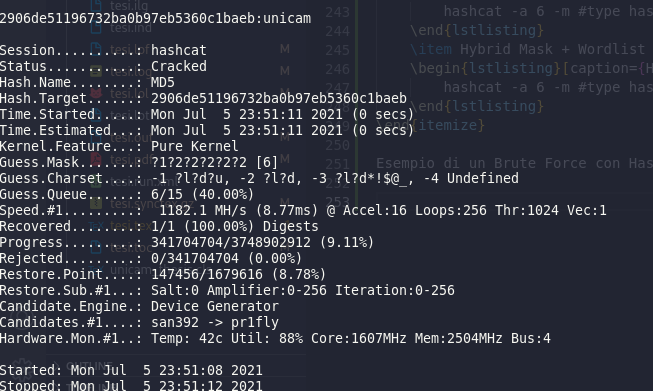
\includegraphics[width=100mm]{Immagini/1/hashcat_show.png}
	\caption{hashcat example}
    \label{fig:hashcat example}
\end{figure}
\chapter{Extract Hashes}
Una parte fondamentale dei attacchi Brute Force è il fatto di recuperare gli hash, in modo da poterli attaccare offline, andando a ridurre così i tempi e le tracce che si possono lasciare.
Questi hash possono trovarsi in vari sistemi, diversi tra loro e ognuno si differenzia per il modo e per i strumenti con cui si possono recuperare.
\section{Windows}
In Windows gli hash inerenti alle password degli account, sono archiviati in un file di un database nel controller di dominio (NTDS.DIT) con alcune informazioni aggiuntive come le appartenenze ai gruppi e gli utenti.

Il file NTDS.DIT è costantemente utilizzato dal sistema operativo e quindi non può essere copiato direttamente in un'altra posizione per l'estrazione delle informazioni.
\begin{lstlisting}[ caption={NTDS.DIT Directory}, style=javaScriptCode]
    C:\Windows\NTDS\NTDS.dit
\end{lstlisting}

Esistono varie tecniche che possono essere utilizzate per estrarre questo file o le informazioni memorizzate al suo interno.

\subsection{CREDDUMP}

Questo strumento\cite{CREDDUMP} permette di estrarre ogni possibile cache delle credenziali dei domini.

Prima di tutto dobbiamo creare una copia dei registri di Windows:

\begin{lstlisting}[ caption={Copy reg.}, style=javaScriptCode]
    C:\WIND0WS\system32>reg.exe save HKLM\SAM sam_backup.hiv
    C:\WIND0WS\system32>reg.exe save HKLM\SECURITY sec_backup.hiv
    C:\WIND0WS\system32>reg.exe save HKLM\system sys_backup.hiv
    \end{lstlisting}


Successivamente possiamo utilizzare tre tipi di attacchi :
\begin{itemize}
    \item cachedump -> scarica le credenziali memorizzate nella cache
          \begin{lstlisting}[ caption={Cachedump esempio}, style=javaScriptCode]
        root@kali:~# cachedump
                     usage: /usr/bin/cachedump <system hive> <security hive>
                     cachedump sys_backup.hiv sec_backup.hiv
    \end{lstlisting}
    \item lsadump -> scarica le credenziali LSA
          \begin{lstlisting}[ caption={Lsadump esempio}, style=javaScriptCode]
        root@kali:~# lsadump
                     usage: /usr/bin/lsadump <system hive> <security hive>
                     lsadump sys_backup.hiv sec_backup.hiv
    \end{lstlisting}
    \item pwdump -> scarica gli hash della password
          \begin{lstlisting}[ caption={Pwdump esempio}, style=javaScriptCode]
        root@kali:~# pwdump 
                     usage: /usr/bin/pwdump <system hive> <security hive>
                     pwdump sys_backup.hiv sec_backup.hiv 
    \end{lstlisting}
\end{itemize}

\subsection{MIMIKATZ}

Mimikatz\cite{MIMIKATZ}, creato da gentilkiwi , può essere utilizzato per estrarre hash di password e codici PIN dalla memoria di Windows.

Oggi, Windows Defender e i software di antivirus sono diventati sempre più efficaci nel rilevare le esecuzioni e le firme di Mimikatz.


\begin{figure}[h!]
    \centering
    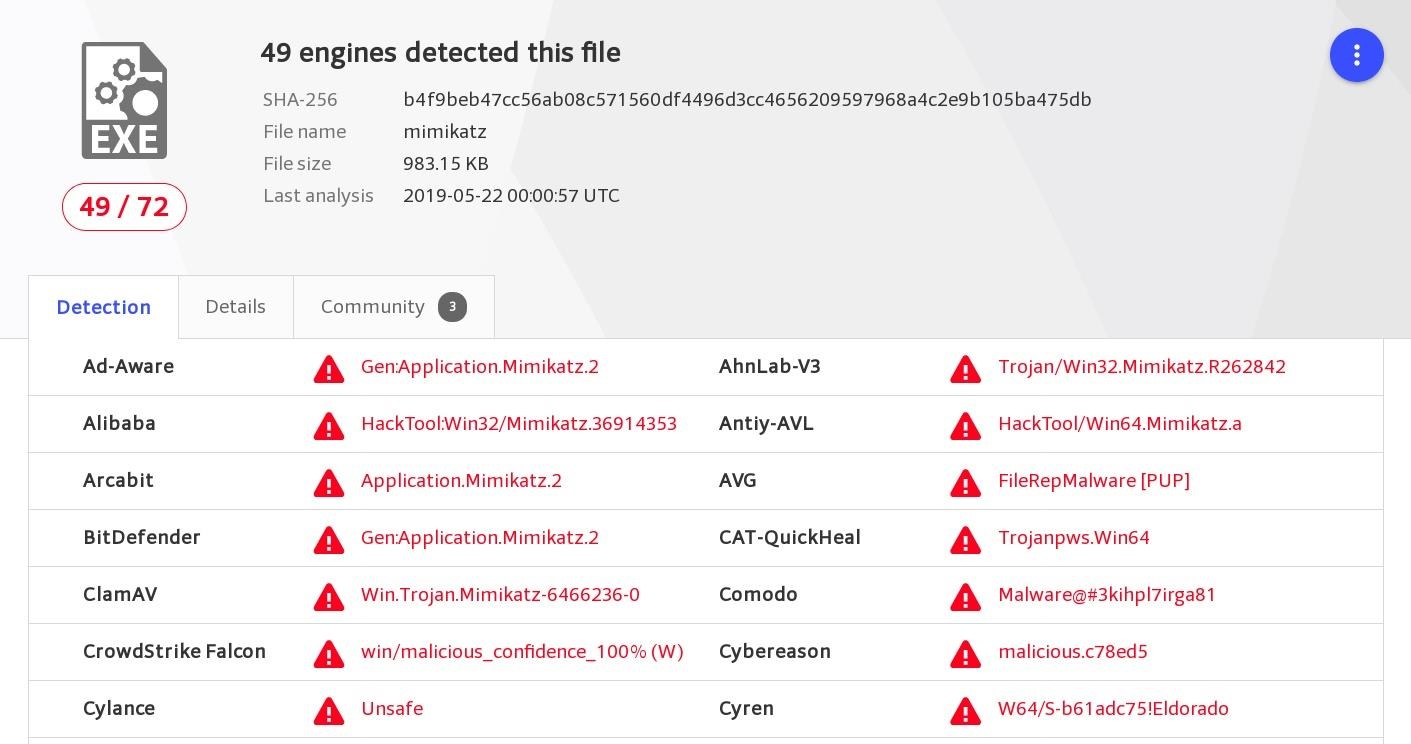
\includegraphics[width=120mm]{Immagini/2/mimikatz.jpg}
    \caption{MIMIKATZ e antivirus}
    \label{fig:MIMIKATZ}
\end{figure}

In combinazione con Mimikatz ora si utilizza ProcDump\cite{ProcDump}, un eseguibile autonomo progettato per gli amministratori per monitorare i crash dump delle applicazioni. ProcDump viene utilizzato per estrarre il dump LSASS\cite{lsass}, ossia Local Security Authority Subsystem Service (LSASS) è un processo nei sistemi operativi Microsoft Windows che è responsabile dell'applicazione della politica di sicurezza nel sistema, verifica gli utenti che accedono a un computer o server Windows, gestisce le modifiche alla password e crea token di accesso e scrive anche nel registro di sicurezza di Windows, questo dump LSASS viene successivamente spostato su un computer Windows offline e analizzato con Mimikatz . Questa è ancora una tecnica efficace per estrarre le credenziali da Windows, poiché ProcDump è un binario Microsoft firmato e non viene segnalato dalla maggior parte dei software antivirus.

\begin{figure}[h!]
    \centering
    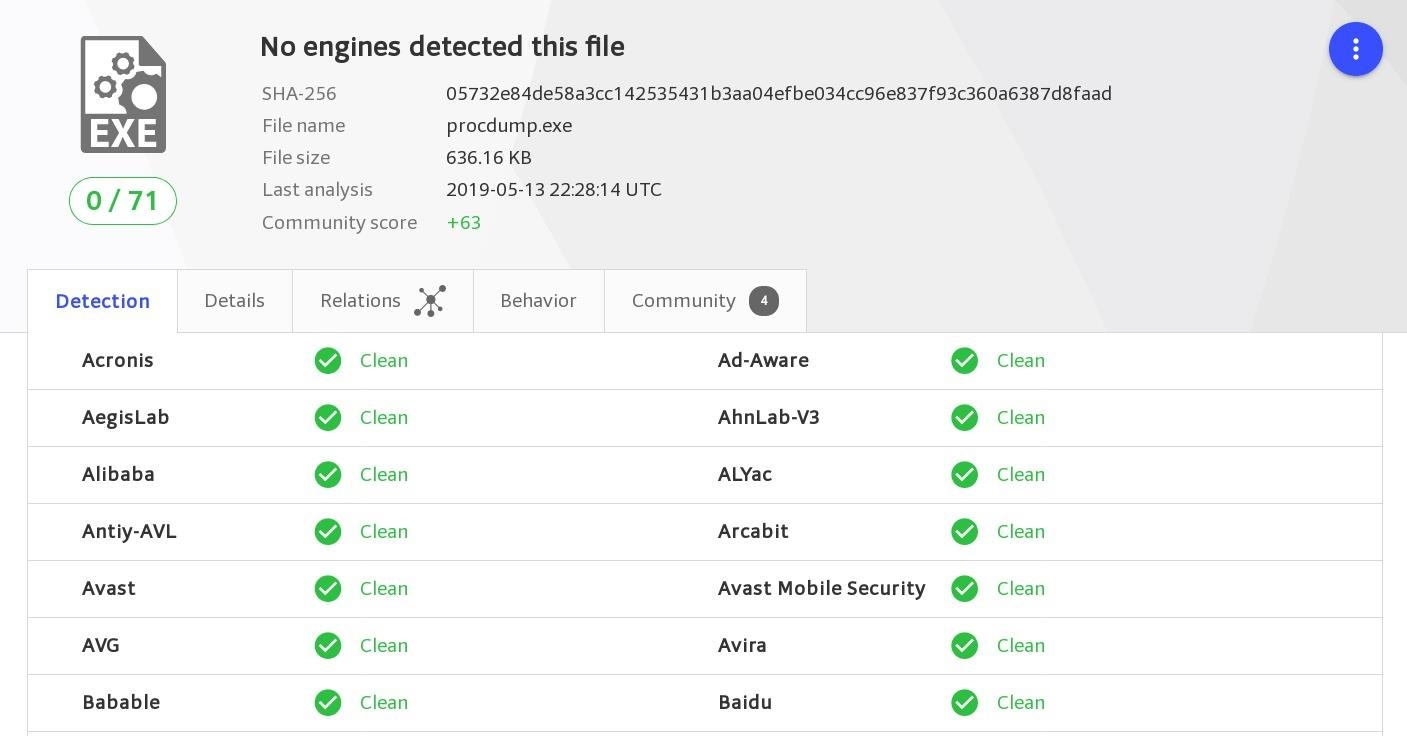
\includegraphics[width=120mm]{Immagini/2/procdump.jpg}
    \caption{ProcDump e antivirus}
    \label{fig:ProcDump}
\end{figure}

\newpage

Per eseguire il Dump, basta digitare il seguente comando (una volta scaricato procDump) nel prompt dei comandi :

\begin{lstlisting}[ caption={ProcDump copia lsass}, style=javaScriptCode]
    C:\procdump.exe -accepteula -ma lsass.exe lsass.dmp
\end{lstlisting}

Una volta svolto il Dump con procDump e spostato il file nella macchina che eseguirà l'attacco, possiamo passare a Mimikatz. 
Apriamo mimikatz con i permessi di amministratore.
\begin{figure}[h!]
    \centering
    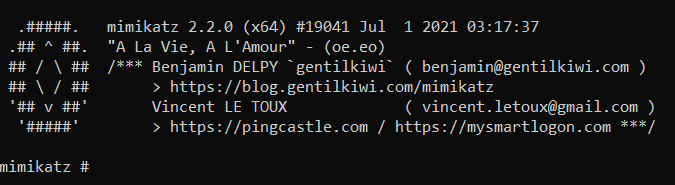
\includegraphics[width=100mm]{Immagini/2/mimikatz_1.PNG}
    \caption{Mimikatz primo avvio}
    \label{fig:ProcDump}
\end{figure}

Ora abilitiamo il log e andiamo a spostare lo spazio di lavoro di mimikatz sul file generato da procDump 

\begin{figure}[h!]
    \centering
    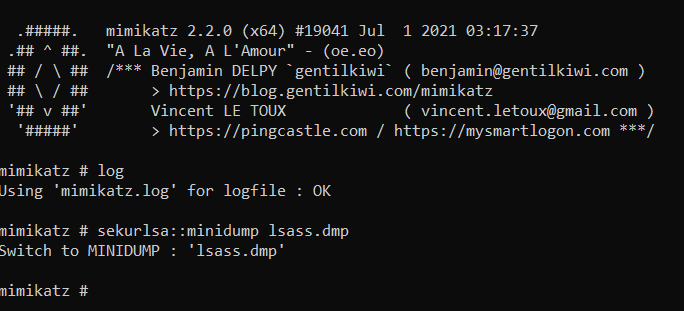
\includegraphics[width=100mm]{Immagini/2/mimikatz_2.PNG}
    \caption{Mimikatz setup}
    \label{fig:ProcDump}
\end{figure}

\begin{lstlisting}[ caption={Mimikatz command setup}, style=javaScriptCode]
    log
    sekerlsa::minidump lsass.dmp
\end{lstlisting}

Ora siamo pronti per recuperare tutte le password memorizzate internamente al sistema, eseguendo il seguente comando :

\begin{lstlisting}[ caption={Mimikatz Logon Passwords}, style=javaScriptCode]
    sekerlsa::logonpasswords
\end{lstlisting}

\begin{figure}[h!]
    \centering
    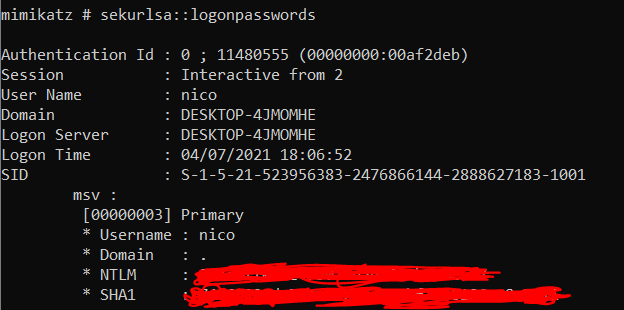
\includegraphics[width=100mm]{Immagini/2/mimikatz_3.PNG}
    \caption{Mimikatz dumo hash}
    \label{fig:ProcDump}
\end{figure}

Una volta recuperati gli hash delle password siamo pronti per eseguire un Brute Force attraverso per esempio lo strumento hashcat o john the ripper.


\section{Linux}

Un attaccante su un sistema Linux\cite{hash_Linux}, per prima cosa se ha i permessi di root, andrà vedere all'interno della cartella \textbf{ETC/SHADOW}

\begin{figure}[h!]
    \centering
    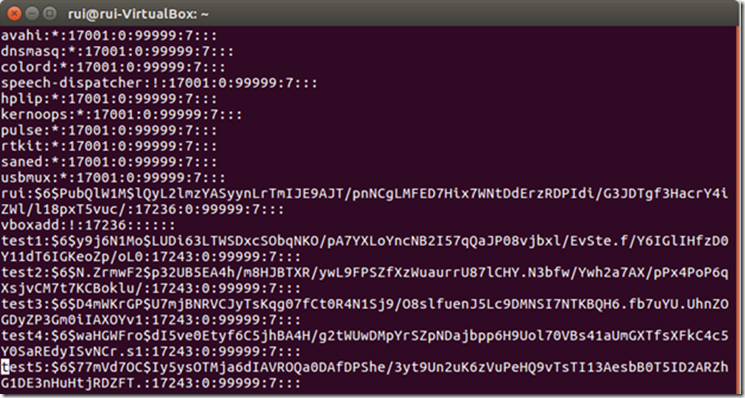
\includegraphics[width=100mm]{Immagini/2/linux_1.png}
    \caption{ETC/SHADOW}
    \label{fig:ProcDump}
\end{figure}

\begin{lstlisting}[ caption={ETC/SHADOW}, style=javaScriptCode]
    root@kali:~# cat etc/shadow
\end{lstlisting}

Eseguendo questo comando sarà possibile ottenere informazioni sulle password degli utenti del sistema.

Ogni riga di questo file contiene nove campi suddivisi in 

\begin{lstlisting}[ caption={ETC/SHADOW composizione}, style=javaScriptCode]
mark:$6$.n.:17736:0:99999:7:::
[--] [----] [---] - [---] ----
|      |      |   |   |   |||+-----------> 9. Inutilizzato
|      |      |   |   |   ||+------------> 8. Data di scadenza
|      |      |   |   |   |+-------------> 7. Periodo di inattivita
|      |      |   |   |   +--------------> 6. Periodo per la scadenza
|      |      |   |   +-----------------> 5. Eta massima della password
|      |      |   +--------------------> 4. Eta minima della password
|      |      +-----------------------> 3. Ultima modifica della password
|      +----------------------------> 2. Password crittografata ($1$ -MD5, ecc ecc)
+----------------------------------> 1. Username
\end{lstlisting}

Vediamo un esempio :

\begin{lstlisting}[ caption={ETC/SHADOW esempio}, style=javaScriptCode]
    mario:$1$bgfrJMa5U384smbQ$z6nch...:18009:0:120:7:14::
\end{lstlisting}

La linea sopra contiene le informazioni dell'utente "Mario"

\begin{itemize}
    \item La password è crittografata con SHA-512 (la password viene troncata per una migliore leggibilità).
    \item La password è stata modificata l'ultima volta il 23 aprile 2019 - 18009.
    \item Non esiste un'età minima per la password.
    \item La password deve essere cambiata almeno ogni 120 giorni.
    \item L'utente riceverà un messaggio di avviso sette giorni prima della data di scadenza della password.
    \item Se l'utente non tenta di accedere al sistema 14 giorni dopo la scadenza della password, l'account verrà disabilitato.
    \item Non esiste una data di scadenza dell'account.
\end{itemize}

Su Linux, inoltre è possibile recuperare le informazioni inerenti le password anche in altre directory come :

\begin{itemize}
    \item /home/*/./bash\_history
    \item /home/*/.mysql\_history
    \item /etc/cups/printers.conf
    \item /home/*/.ssh/
    \item /tmp/krb5cc\_*
    \item /home/*/.gnupg/secring.gpgs
\end{itemize}

\subsection{File}

Un'altra operazione possibile è quella di recuperare gli hash delle password dei file protetti. Questo tipo di operazione è possibile grazie allo strumento John The Ripper.

John The Ripper mette a disposizione un set di strumenti per estrarre gli hash delle password di diversi tipi di file, ecco riportati alcuni di questi strumenti :


\begin{table}[htbp]
    \begin{center}
    \begin{tabular}{|l|l|}
    \hline
    \textbf{Nome} & \textbf{Descrizione} \\
    \hline
    1password2john.py & estrazione hash 1Password \\
    \hline
    7z2john.py & estrazione hash 7zip \\
    \hline
    bitcoin2john.py & estrazione hash da vecchi wallet Bitcoin \\
    \hline
    blockchain2john.py & estrazione wallet da Blockchain \\
    \hline
    rar2john & estrazione hash da RAR 3.x \\
    \hline
    office2john.py & estrazione hash da file Microsoft Office \\
    \hline
    pdf2john.py & estrazione hash da PDF criptati \\
    \hline
    ssh2john & estrazione chiavi SSH private \\
    \hline
    zip2john & processa ZIP file per estrarre hash nel formato JTR \\
    \hline
    

    \end{tabular}
    \end{center}
    \caption{John The Ripper estrazione hash da file}
    \label{tab:browser}
    \end{table}

    Ecco un esempio:

    Si ha un file ZIP criptato con la seguente chiave : "ciao".

    Per prima cosa dobbiamo andare ad estrarre l'hash della password da questo e salvarla su di un'altro file. Per fare questo andremo ad utilizzare il comando \textbf{zip2john}.

    \begin{lstlisting}[ caption={Estrazione hash da file zip}, style=javaScriptCode]
        root@kali:~# zip2john file.zip > output.txt
    \end{lstlisting}

    \begin{figure}[h!]
        \centering
        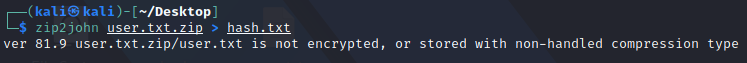
\includegraphics[width=\linewidth]{Immagini/3/hash_ex.png}
        \caption{Estrazione hash da file zip}
    \end{figure}

    Una volta recuperato l'hash della password del file, possiamo passare ad eseguire il Brute Force su di questo. Per recuperare la password useremo sempre John The Ripper, andando però a specificare il formato del file da cui è stato estrapolato, per fare questo aggiungeremo il parametro \textbf{--format}.  

    \begin{lstlisting}[ caption={Conversione hash file zip nella password}, style=javaScriptCode]
        root@kali:~# sudo john --format=zip hash.txt
    \end{lstlisting}

    \begin{figure}[h!]
        \centering
        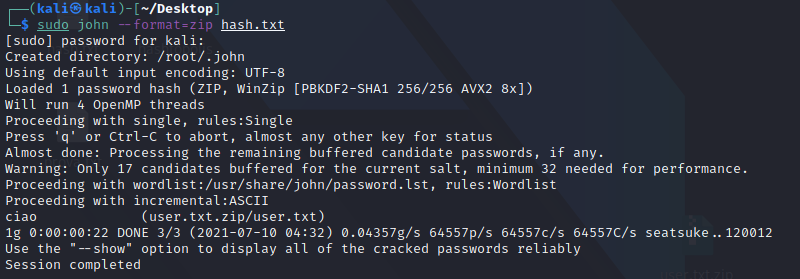
\includegraphics[width=\linewidth]{Immagini/3/hash_ex_2.png}
        \caption{Conversione hash file zip nella password}
    \end{figure}
\chapter{Brute Force Dispositivi mobile}
In questo capitolo andremo a discutere di come viene eseguito un Brute Force sui dispositivi mobile.

\section{Brute Force con Dispositivi mobile}

Una delle metodologie possibili da applicare per eseguire un Brute Force sui dispositivi mobile è quella di utilizzare un'altro device mobile per eseguire l'attacco, questo è possibile grazie all'installazione di NetHunter sul device attaccante, un sistema operativo che ci permetterà di abilitare determinate operazioni eseguibili sul dispositivo.

\subsection{NetHunter}

NetHunter\cite{NetHunter} è una ROM per Android sviluppata appositamente per chi vuole utilizzare i programmi presenti nella distribuzione Kali Linux da telefono.

NetHunter permette quindi di interfacciarsi con i vari strumenti per testare la sicurezza informatica. Nei software a disposizione si troveranno diversi programmi per effettuare attacchi di tipo HID Keyboard, BadUSB, Evil AP MANA e molto altro. 

Kali NetHunter è disponibile per dispositivi senza root (NetHunter Rootless), per dispositivi rooted (NetHunter Lite / NetHunter).

\begin{figure}[h!]
    \centering
    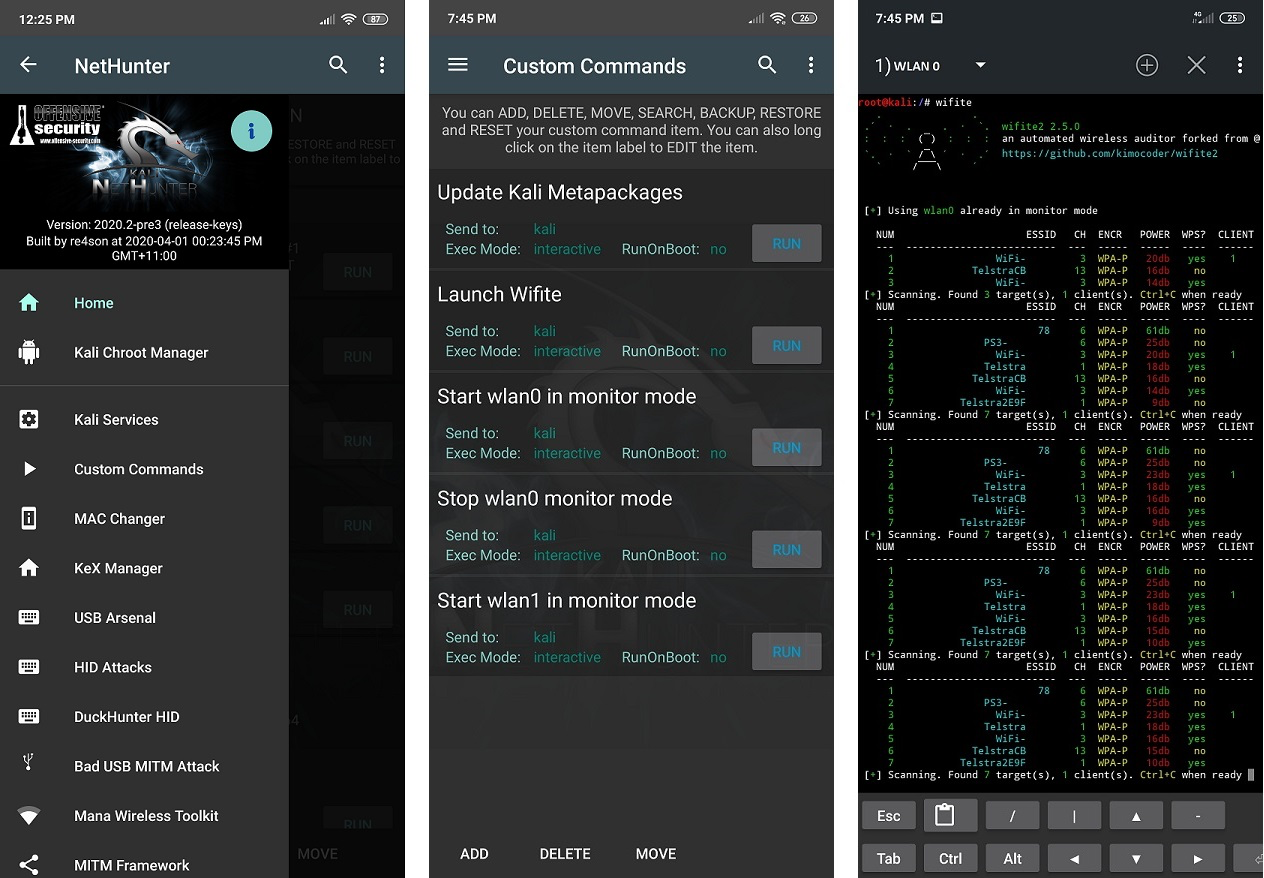
\includegraphics[width=116mm]{Immagini/3/nethunter_1.png}
    \caption{NetHunter}
    \label{fig:NetHunter}
\end{figure}

\newpage

Nel nostro caso andremo ad utilizzare la versione NetHunter, che ci permetterà di utilizzare l'interfaccia HID\footnote[1]{\textbf{HID} : Human Interface Device o HID è un tipo di dispositivo informatico solitamente utilizzato dagli esseri umani che riceve input dagli umani e fornisce output agli umani.}, questa permetterà al dispositivo attaccante di comunicare con il dispositivo vittima, come se fosse un mouse o una tastiera.

\subsection{Android-PIN-Bruteforce}

La prima tecnica che andremo a vedere è Android-PIN-Bruteforce\cite{Android-PIN-Bruteforce} che è stato sviluppato dal gruppo urbanadventur, qui si andrà a sfruttare l’interfaccia HID per simulare l’utilizzo di una tastiera per l’inserimento dei PIN, permettendo di provare tutti i PIN possibili in circa 16 ore.

Per eseguire questo tipo di attacco dobbiamo essere in possesso di un dispositivo mobile che sia compatibile per via ufficiali\cite{nethunter_official} o mantenuto dalla community\cite{nethunter_community}. Una volta che si ha il dispositivo bisogna installare Nethunter su di esso in modo da abilitare l'interfaccia HID.

L'ultima due cose necessarie per eseguire l'attacco sono un cavo OTG (maschio micro USB  -> femmina USB-A) e il dispositivo vittima con il suo cavo di ricarica.

\begin{figure}[h!]
    \centering
    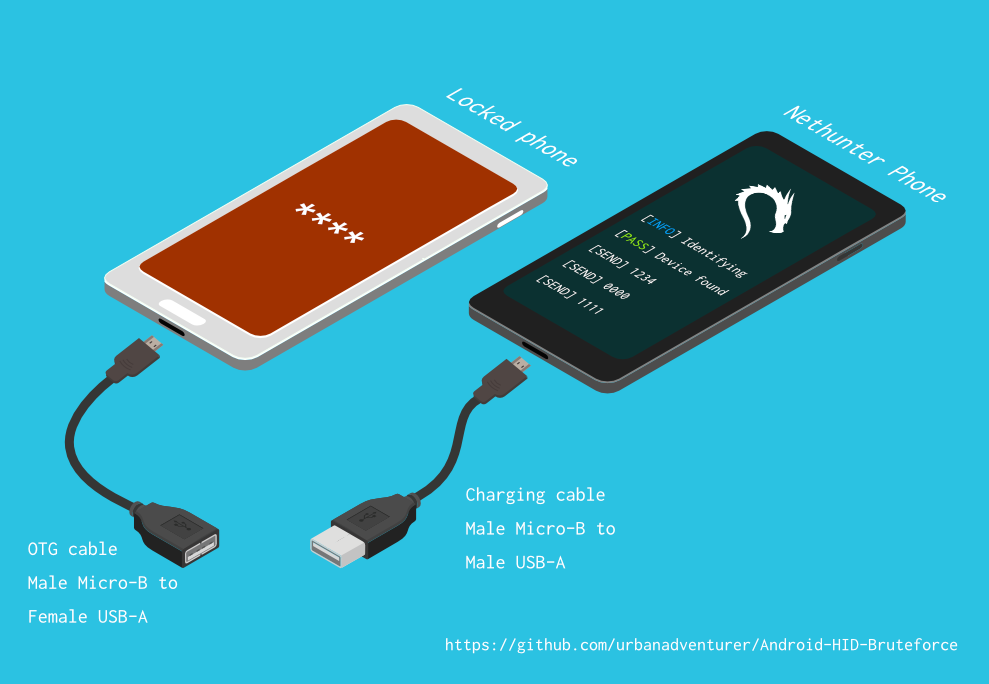
\includegraphics[width=140mm]{Immagini/3/pin_brute_1.png}
    \caption{Android-PIN-Bruteforce}
    \label{fig:Android-PIN-Bruteforce}
\end{figure}

Questa tecnica permette di :
\begin{itemize}
	\item A differenza di altri metodi, non è necessario abilitare il debug ADB o USB sul telefono bloccato, inoltre si può impostare la lunghezza della password da provare (da 1 a 10).
	\item Il telefono Android bloccato non ha bisogno di essere rootato
	\item Trasforma il tuo telefono NetHunter in una macchina per crackare il PIN Android
	\item Non è necessario acquistare hardware speciale
	\item Utilizza i file di configurazione per supportare diversi telefoni
	\item Elenchi di PIN ottimizzati per PIN a 3,4,5 e 6 cifre
	\item Ignora i popup del telefono incluso l’avviso di basso consumo
	\item Rileva quando il telefono è scollegato o spento e attende mentre riprova ogni 5 secondi
	\item Ritardi configurabili di N secondi dopo ogni X tentativi di PIN
\end{itemize}

Per eseguire il seguente script, basta scaricarlo dal git ufficiale del gruppo e collegare il dispositivo attaccante al dispositivo vittima come detto in precedenza e lanciare dal terminale del dispositivo il comando :

\begin{lstlisting}[ caption={Android-PIN-Bruteforce command}, style=javaScriptCode]
	bash ./android-pin-bruteforce crack
\end{lstlisting}

\begin{figure}[h!]
    \centering
    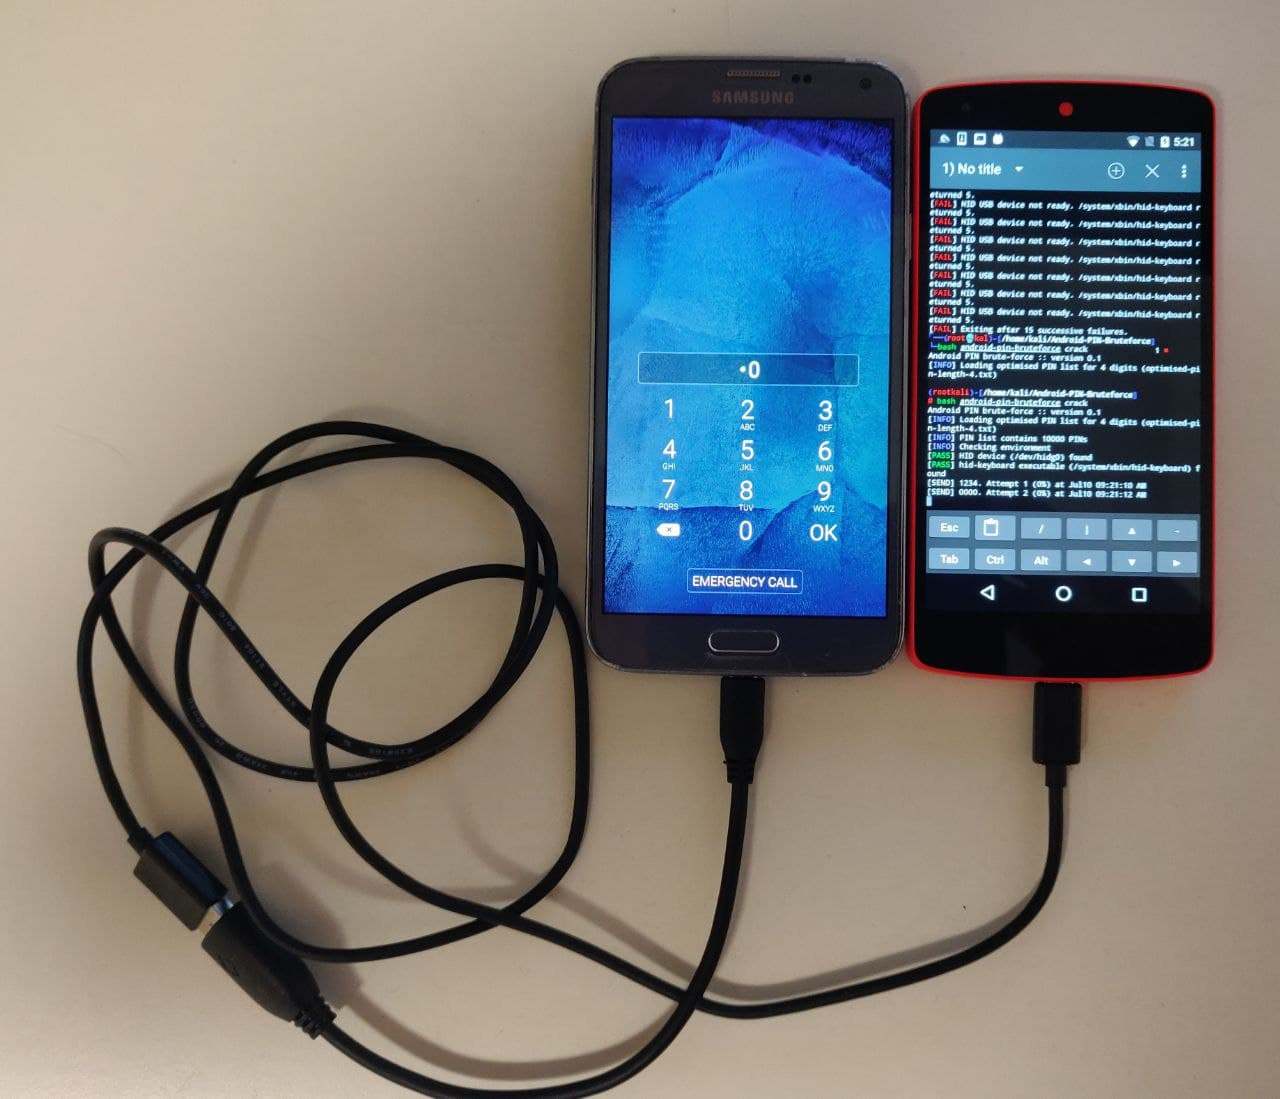
\includegraphics[width=140mm]{Immagini/3/brute.jpg}
    \caption{Android-PIN-Bruteforce esempio}
    \label{fig:Android-PIN-Bruteforce}
\end{figure}

Questo script come detto, fa uso di una serie di liste di PIN ottimizzate (Gli elenchi di PIN ottimizzati sono stati generati estraendo le password numeriche dalle perdite di database e quindi ordinandole in base alla frequenza). Per la scelta della lunghezza dei PIN da utilizzare, basta aggiungere il comando –length X, dove X sta per la lunghezza della password da utilizzare.

Inoltre è possibile utilizzare delle maschere per i PIN da utilizzare :
\begin{itemize}
	\item Per provare tutti gli anni dal 1900 al 1999 \newline
	\begin{lstlisting}[ caption={Android-PIN-Bruteforce command mask}, style=javaScriptCode]
		bash ./android-pin-bruteforce crack -mask "19.."
	\end{lstlisting}
	\item Per provare i PIN che hanno un 1 nella prima cifra e un 1 nell’ultima cifra \newline
	\begin{lstlisting}[ caption={Android-PIN-Bruteforce command maSsk}, style=javaScriptCode]
		bash ./android-pin-bruteforce crack -mask "1..1"
	\end{lstlisting}
	\item Per provare i PIN che terminano con 4 o 5, usa \newline
	\begin{lstlisting}[ caption={Android-PIN-Bruteforce command mask}, style=javaScriptCode]
		bash ./android-pin-bruteforce crack -mask ...[45]
	\end{lstlisting}
\end{itemize}

I produttori di dispositivi creano le proprie schermate di blocco diverse da quelle predefinite o di serie di Android, per specificare una predefinita configurazione, bisogna aggiungere il comando –config ConfingFile, che permette di adattare i comandi inviati in base alla configurazione del dispositivo vittima.

Una funzione importante è il fatto che il dispositivo attaccante in automatico ogni X tentativi si metterà in pausa, simulando il time out dovuto ai vari tentativi falliti.

\begin{figure}[h!]
    \centering
    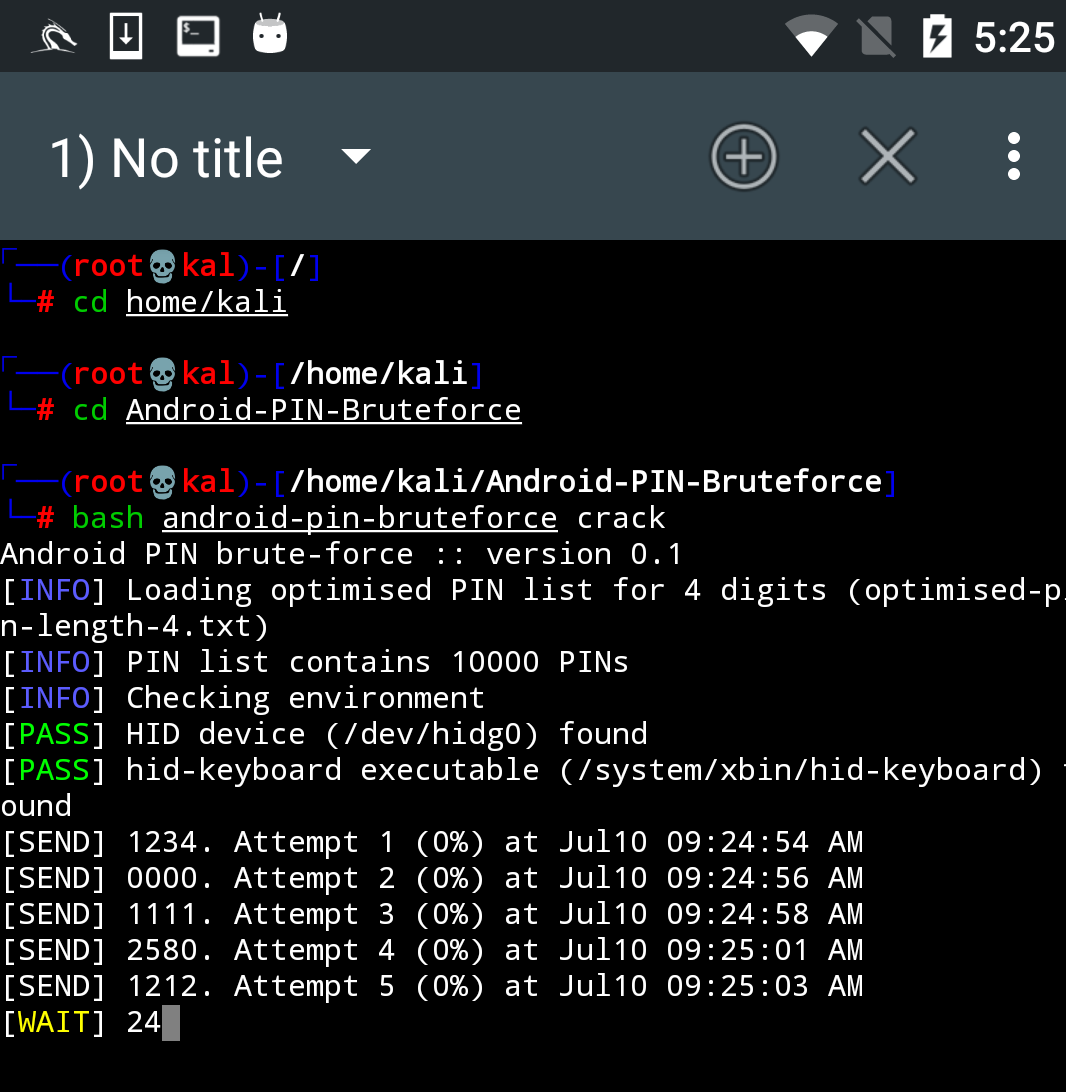
\includegraphics[width=80mm]{Immagini/3/Screenshot_20210710-052513.png}
    \caption{Android-PIN-Bruteforce time out}
    \label{fig:Android-PIN-Bruteforce}
\end{figure}

Una delle problematiche di questo script è il fatto che non sia in grado di riconoscere quando il PIN che abbiamo utilizzato avrà successo, infatti lui, anche dopo aver sbloccato il dispositivo continuerà con i vari tentativi.

\section{WBRUTE}

Un’altra tecnica testata è quella WBRUTE\cite{wbrute}, sviluppata da wuseman. Questa è molto diversa e molto più potente da quella vista in precedenza, per diversi fattori :

\begin{itemize}
	\item Funzionante solo se il dispositivo vittima ha una versione Android 8.0
	\item Permette di bypassare il time out dopo X tentativi errati
	\item Deve essere abilitato ADB nel dispositivo vittima
	\item Deve essere dato l’accesso al dispositivo attaccante dal dispositivo vittima
	\item Permette di sapere il PIN corretto
	\item Permette di sostituire il PIN con uno nuovo
	\item Utilizzabile con PIN di 4 o 6 cifre
	\item Il dispositivo vittima deve essere rootato
\end{itemize}

Questa tecnica sfrutta una vulnerabilità introdotto con Android 8.0, nata dalla rimozione della possibilità di impostare come PIN l’orario attuale, per un errore è stato lasciato il comando locksettings che permette di eseguire operazioni sul PIN, in questo caso di proverà a rimuovere il PIN corretto, andando a catturare il messaggio di successo in modo da avere una conferma che il PIN sia corretto.

\begin{figure}[h!]
	\centering
	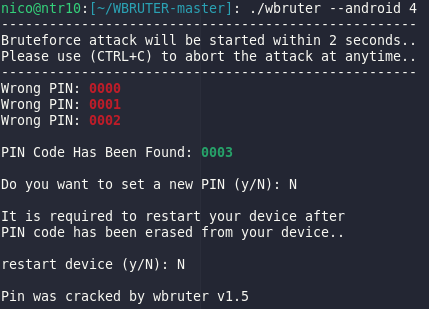
\includegraphics[width=100mm]{Immagini/3/wbrute.png}
	\caption{WBRUTE esempio}
    \label{fig:WBRUTE_esempio}
\end{figure}

Il comando eseguito è :

\begin{lstlisting}[ caption={Android-PIN-Bruteforce command}, style=javaScriptCode]
	adb shell locksettings clear -old $i | grep "Lock credential cleared"
\end{lstlisting}

Dove \$i è il valore che verrà testato (da 0000 a 9999). Una volta trovato il PIN questo ci verrà mostrato a schermo sul device attaccante e richiesto se si vuole modificare con un’altro. Questa tecnica permette di provare tutti e 9999 PIN in poco più di un’ora grazie al fatto che non si ha il problema del time out, ma come detto in precedenza, questa tecnica è poco applicabile, per il fatto che si deve avere un dispositivo bloccato con Android 8.0, debug USB attivo e autorizzazione per il device attaccante.

Il tutto è Funzionante grazie allo strumento adb\cite{adb} che permette l’esecuzione di comandi direttamente sul dispositivo.


\section{CiLocks}

CiLocks\cite{CiLocks} è un'altro strumento utilizzato per eseguire il Pin brute force su dispositivi mobile, questo come Android-PIN-Bruteforce permette l'utilizzo di dizionari personalizzati ed inoltre permette di unire diverse tecniche, come quella vista in WBRUTE.

\begin{figure}[h!]
	\centering
	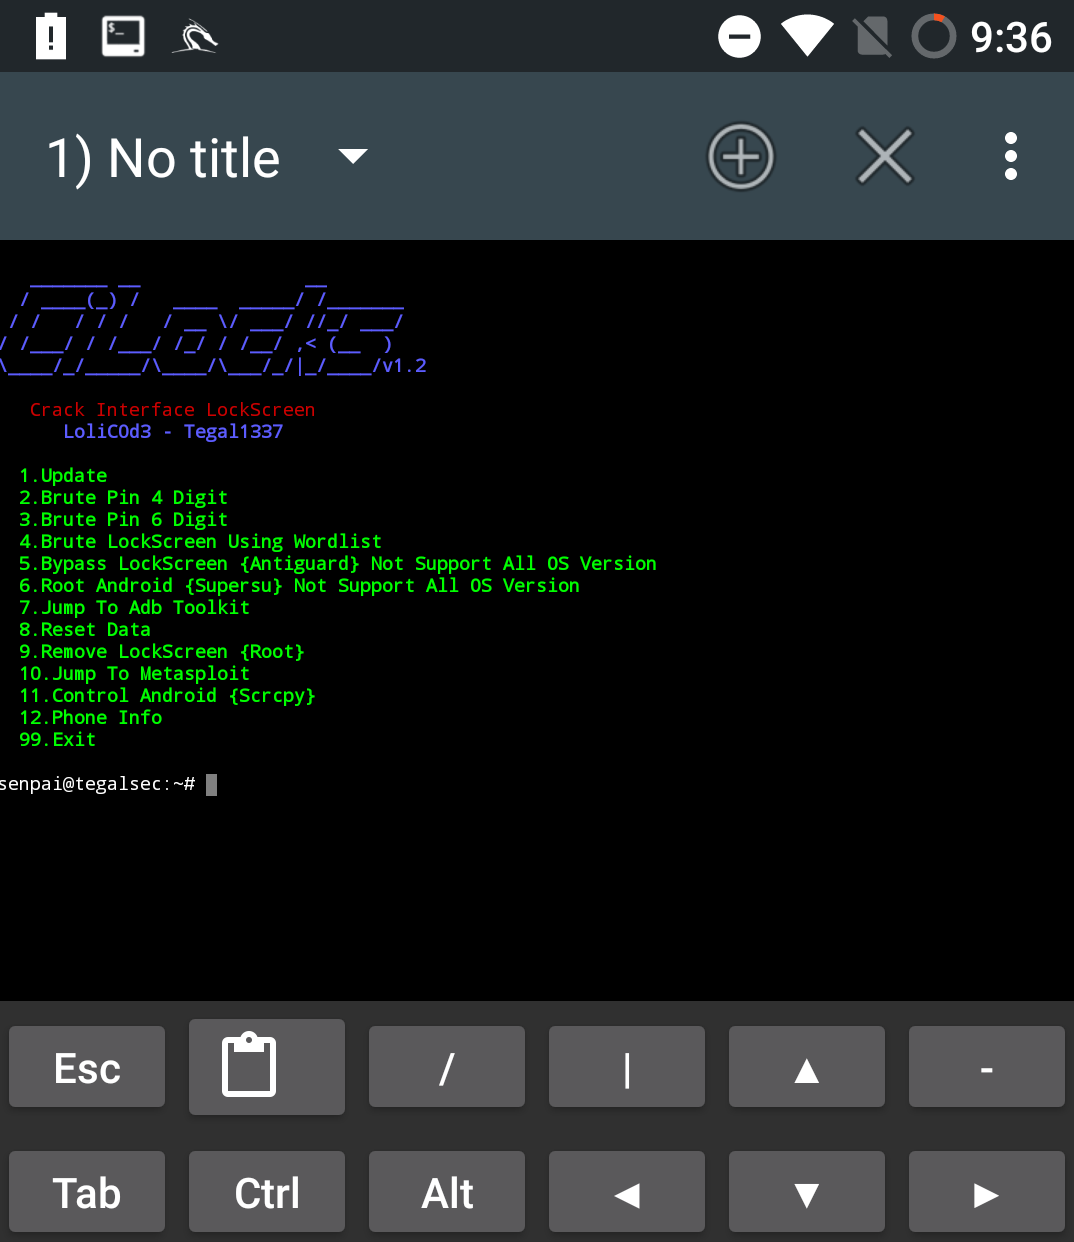
\includegraphics[width=100mm]{Immagini/3/cilocks.png}
	\caption{CiLocks esempio}
    \label{fig:CiLocks_esempio}
\end{figure}
\chapter{Wi-Fi Brute Force}
\section{Tecniche}
\section{Strumenti}
\section{Esempio}
\label{chap:conc}

\chapter{Wi-Fi Brute Force}

Un Brute Force su di una rete Wi-Fi, per prima cosa dobbiamo riuscire a catturare l'handshake che avviene tra il punto di accesso alla rete e il client, in questo handshake possiamo trovare informazioni inerenti alla password.

Per eseguire questo tipo di attacco, un malintenzionato ha addisposizione molti strumenti : Aircrack-ng, Fern, Wifite, AirJack, ecc ecc . Ora andremo a vedere nel dettaglio alcuni di questi strumenti.

\section{Aircrack-ng}

Aircrack-ng\cite{aircrack} è uno strumento utilizzato per valutare la sicurezza delle rete Wi-Fi. Questo tool si compone di una suite di strumenti, ognuno con un proprio scopo :
\begin{itemize}
    \item \textbf{Airmon-ng} utilizzato per impostare l'interfaccia di rete in monitor mode. 
    \item \textbf{Airodump-ng} utilizzato per acquisire i pacchatti di autenticazione Wi-Fi.
    \item \textbf{Aireplay-ng} utilizzato per eseguireun iniezione di frame al fine di generare traffico nella rete.
    \item \textbf{Aircrack-ng} utilizzato per violare le password Wi-Fi.
\end{itemize}

Per eseguire questo tipo dia attacco abbiamo bisogno di una particolare scheda di rete, questa deve supportare la monitor mode\footnote[1]{\textbf{monitor mode} : permette di catturare i pacchetti nella rete senza doversi connettere ad un access point (questa modalità funziona solo con reti wireless)}.

Successivamente dobbiamo andare a configurare la nostra scheda, quindi utilizzeremo il comando riportato qui sotto per individuare la scheda che andremo ad utilizzare.

\begin{lstlisting}[ caption={Configurazione scheda di rete}, style=javaScriptCode]
	root@kali:~# ip a
\end{lstlisting}

\begin{figure}[h!]
    \centering
    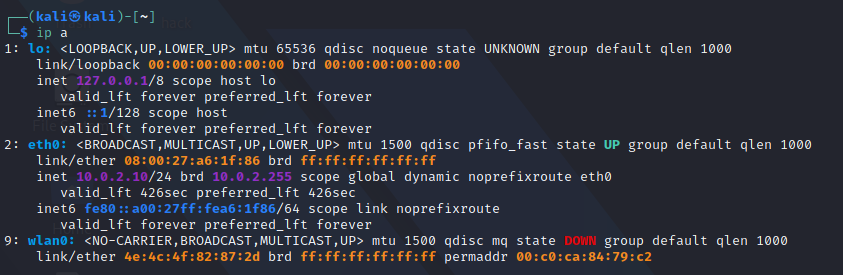
\includegraphics[width=\linewidth]{Immagini/6/aircrack_1.png}
    \caption{Aircrack example}
\end{figure}

\newpage

Una volta individuata la scheda di rete da utilizzare andremo ad eseguire il seguente comando per specificare ad aircrack-ng quale scheda di rete deve utilizzare

\begin{lstlisting}[ caption={Configurazione scheda di rete}, style=javaScriptCode]
	sudo airmon-ng start #nomeschedadirete
\end{lstlisting}

\begin{figure}[ht]
    \centering
    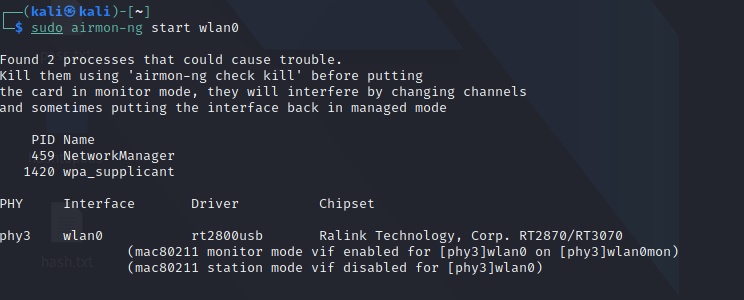
\includegraphics[width=\linewidth]{Immagini/6/aircrack_2.png}
    \caption{Aircrack example}
\end{figure}

Il passo successivo è quello di eseguire una scansione delle reti disponibile, per farlo dobbiamo eseguire il comando :

\begin{lstlisting}[ caption={Scansione delle reti}, style=javaScriptCode]
	sudo airodump-ng wlan0mon
\end{lstlisting}

\begin{figure}[ht]
    \centering
    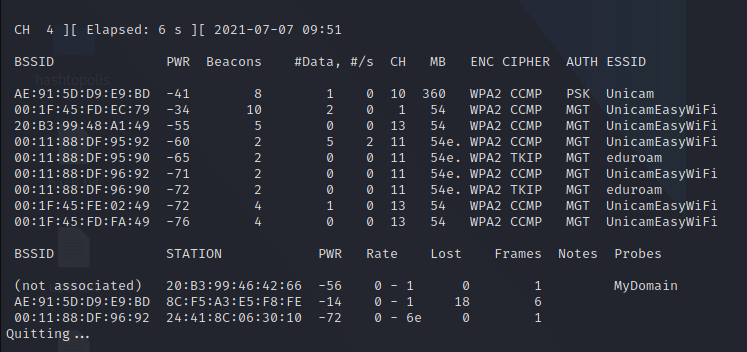
\includegraphics[width=\linewidth]{Immagini/6/aircrack_3.png}
    \caption{Aircrack example}
    \label{fig:Aircrack example}
\end{figure}

\newpage

Dopo aver individuato la rete da attaccare ( in questo caso la rete scelta è Unicam ), dobbiamo salvarci il suo BSSID\footnote[1]{\textbf{BSSID} : Si tratta di un identificatore a 48 bit per il set di servizi di base, è il MAC del lato 802.11 del punto di accesso.} per eseguire un dump dei pacchetti inerenti a quella rete, in modo da poter intercettare i WPA handshake che avvengono tra i client e l'access point. Questi dati verranno memorizzati in un file con estensione .cap\footnote[1]{\textbf{.CAP} : i file con estensione .CAP contengono dati acquisiti dai programmi di tracciamento dei pacchetti. I dati sono in forma grezza, il che significa che vengono salvati nella forma in cui sono stati catturati.} in modo tale da poter eseguire successivamente un Brute Force su questi dati per poterne estrarre la password.

\begin{lstlisting}[ caption={dump dei pacchetti}, style=javaScriptCode]
	sudo airodump-ng --channel 10 --bssid #BSSID_AccessPoint -w #percorso wlan0mon
\end{lstlisting}

\begin{figure}[ht]
    \centering
    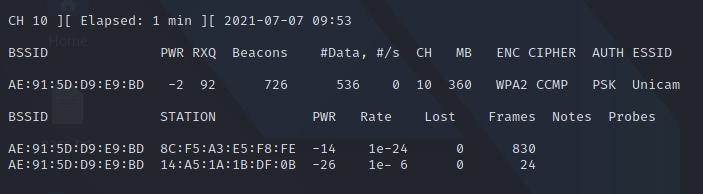
\includegraphics[width=\linewidth]{Immagini/6/aircrack_4.png}
    \caption{Aircrack example}
    \label{fig:Aircrack example}
\end{figure}

Per poter recuperare la password, dobbiamo attendere che venga recuperato il WPA handshake, ma ci potrebbe voler del tempo, quindi una cosa che si può fare è quella di andar a scollegare alcuni utenti dalla rete in modo che cosi debbano ricollegarsi, facendo partire un handshake. Questo è possibile grazie ad aireplay-ng.

\begin{lstlisting}[ caption={aireplay deauth}, style=javaScriptCode]
	sudo aireplay-ng -0 5 -b #BSSID_AccessPoint -h BSSID_Client wlan0mon
\end{lstlisting}

\begin{figure}[ht]
    \centering
    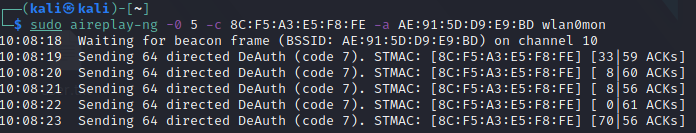
\includegraphics[width=\linewidth]{Immagini/6/aircrack_7.png}
    \caption{Aircrack example}
    \label{fig:Aircrack example}
\end{figure}

Una volta che vediamo che compare la scritta WPA handshake in alto a destra, possiamo chiudere il programma.

\begin{figure}[ht]
    \centering
    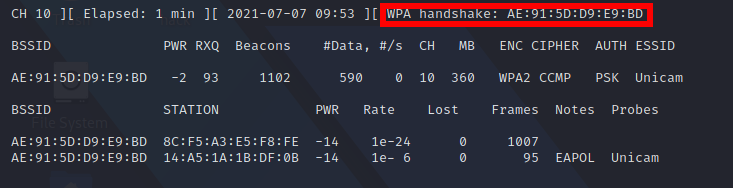
\includegraphics[width=\linewidth]{Immagini/6/aircrack_5.png}
    \caption{Aircrack example}
    \label{fig:Aircrack example}
\end{figure}

Ora che abbiamo recuperato tutti i pacchetti di cui abbiamo bisogno per estrare la password della rete Wi Fi, dobbiamo eseguire un Brute Force su questi dati "grezzi". Per eseguire il Brute Force, possiamo utilizzare il comando aircrack-ng, che permette tramite l'utilizzo di un dizionario, di eseguire un attacco per individuare la password della rete.

\begin{lstlisting}[ caption={aircrack Brute Force}, style=javaScriptCode]
    sudo aircrack-ng -z -b #BSSID_AccessPoint #Path_file_cap -w #Path_Wordlist
\end{lstlisting}

\begin{figure}[ht]
    \centering
    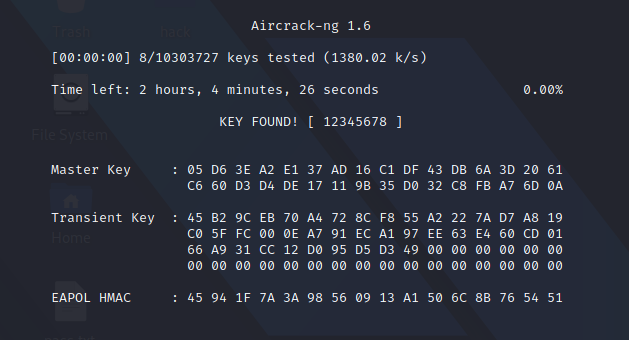
\includegraphics[width=\linewidth]{Immagini/6/ircrack_6.png}
    \caption{Aircrack example}
    \label{fig:Aircrack example}
\end{figure}

\newpage

\section{Fern}

Fern\cite{fern} è un'altro strumento utilizzato per testare la sicurezza delle reti Wi-Fi, come Aircrack. Questo si differenzia per il modo in cui l'utente si interfaccia con il programma, mentre su Aircrack si utilizza un interfaccia a linea di comando, questo strumento ci permette di utilizzare un interfaccia grafica, rendendo l'utilizzo dello strumento più semplice.

\begin{figure}[ht]
    \centering
    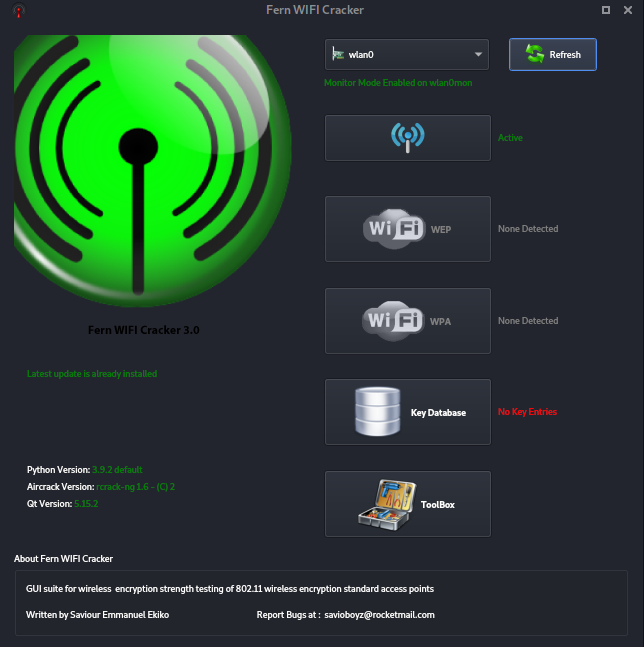
\includegraphics[width=\linewidth]{Immagini/6/fern_1.png}
    \caption{Fern-wifi-cracker}
    \label{fig:Fern example}
\end{figure}

Come possiamo vedere, nella parte superiore possiamo scegliere quale scheda di rete impostare per eseguire la scansione, una volta selezionata la rete possiamo far partire la scansione premendo il tasto sottostante.
\newpage

Una volta avvenuta la scansione, possiamo vedere le reti disponibile suddivise in base al tipo di criptazione, che possono essere o "wifi-wep" o "wifi-wpa", cliccando su uno di questi tasti, possiamo andar a vedere nel dettaglio le reti disponibili. Una volta individuata la rete da attaccare, basterà selezionare la rete, selezionare il dizionario da utilizzare per eseguire l'attacco e premere il tasto \textbf{Attack}.

\begin{figure}[ht]
    \centering
    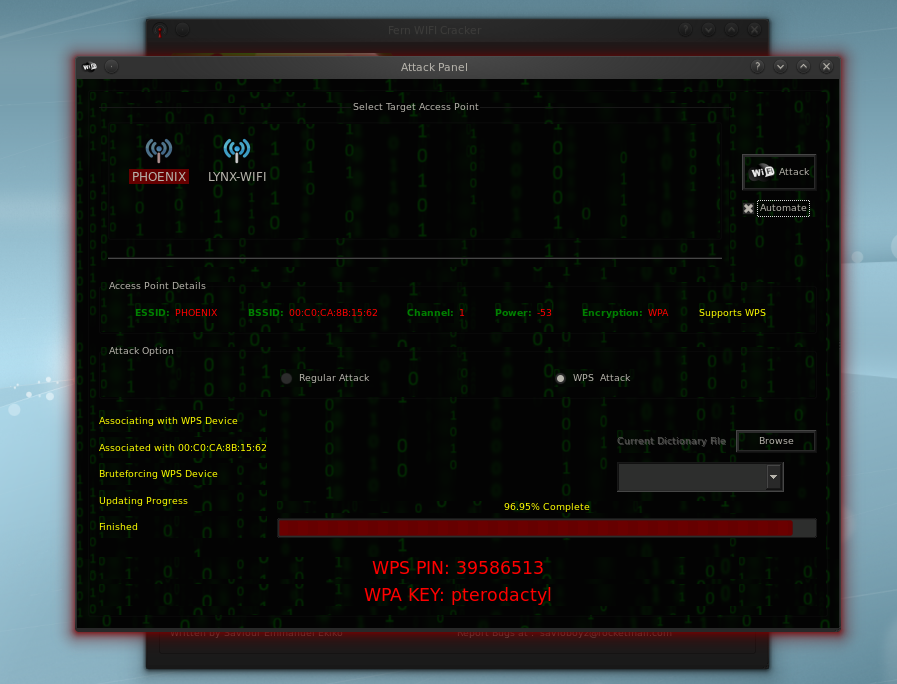
\includegraphics[width=\linewidth]{Immagini/6/fern_3.jpg}
    \caption{Fern-wifi-cracker}
    \label{fig:Fern example}
\end{figure}

\label{chap:conc}

\chapter{CUDA}


\begin{figure}[ht]
    \centering
    
\includegraphics[width=60mm]{Immagini/7/Nvidia_CUDA_Logo.jpg}
    \caption{NVIDIA CUDA logo}
    \label{fig:CPU vs GPU}
\end{figure}

CUDA\cite{hendarto2017performance} (acronimo di Compute Unified Device Architecture) è un'architettura hardware per l'elaborazione parallela creata da NVIDIA. Tramite l'ambiente di sviluppo per CUDA, i programmatori di software possono scrivere applicazioni capaci di eseguire calcolo parallelo sulle GPU delle schede video NVIDIA.

CUDA dà accesso agli sviluppatori ad un set di istruzioni native per il calcolo parallelo di elementi delle GPU CUDA. Usando CUDA, le ultime GPU Nvidia diventano in effetti architetture aperte come le CPU. Diversamente dalle CPU, le GPU hanno un'architettura parallela con diversi core, ognuno capace di eseguire centinaia di processi simultaneamente: se un'applicazione è adatta per questo tipo di architettura, la GPU può offrire grandi prestazioni e benefici.

Dato l'aumentare della complessità dei algoritmi di criptazione nel tempo, questo tipo di tecnologia è diventata molto popolare nell'esecuzione del Brute Force. 

\section{CPU vs GPU}

Diversi tool per il Brute Force ormai permettono l'utilizzo delle GPU insieme alle CPU per eseguire le computazioni per estrarre le password dagli hash. Uno di questi strumenti è Hashcat.

\begin{figure}[ht]
    \centering
    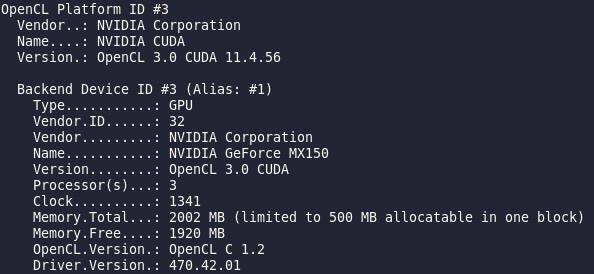
\includegraphics[width=\linewidth]{Immagini/7/GPU_hashcat.png}
    \caption{GPU hashcat}
\end{figure}

\newpage

L'utilizzo della forza computazionale delle GPU, come detto, risulta molto più efficente delle CPU, data la loro possibilità di eseguire operazioni in parallelo, a differenza di delle CPU, che anche se possono avere dai 2 ai 72 core, questi sono ottimizzati per eseguire processi sequenziali, ecco riportati dei esempi (Figura : \ref{fig:CPU vs GPU}) delle differenze delle velocità di calcolo su diversi tipi di algoritmi di criptazione, utilizzando CPU o GPU o entrambi.
\newline

\#1 -> NVIDIA GeForce MX150 - 2048 MB, Core: 1341 MHz, Memoria: 1253 MHz, GDDR5, 382.64, Optimus

\#2 -> Intel Corporation UHD Graphics 620 1.150 MHz

\#3 -> Intel Core i7-8550U CPU @ 1.80GHz

\begin{figure}[ht]
    \centering
    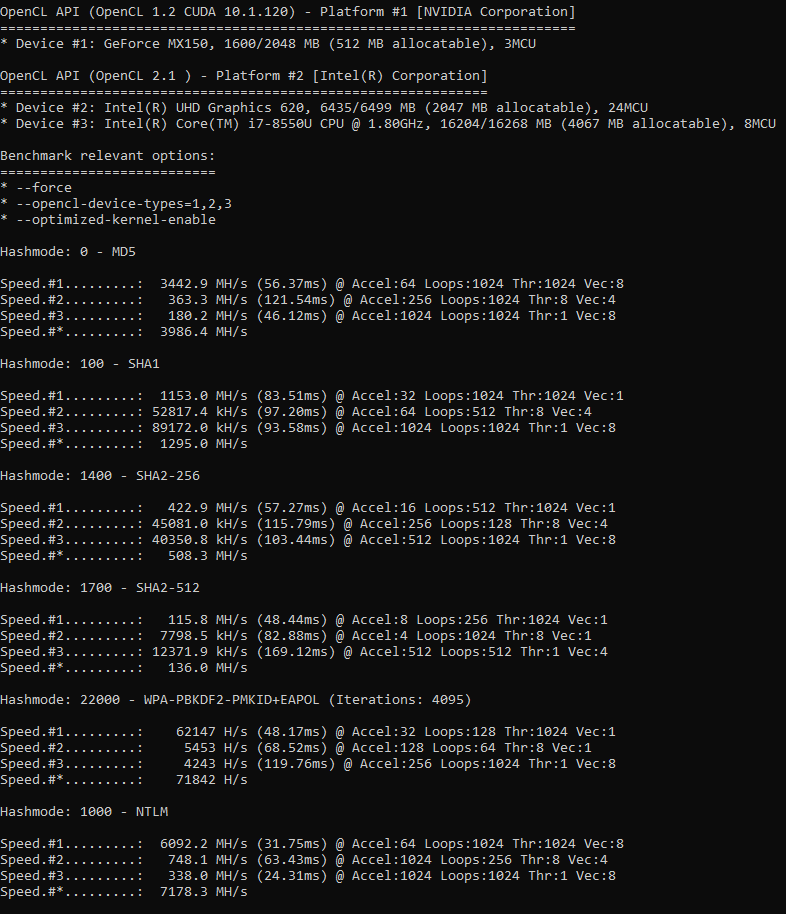
\includegraphics[width=\linewidth]{Immagini/7/cpu_gpu.PNG}
    \caption{CPU vs GPU}
    \label{fig:CPU vs GPU}
\end{figure}

\label{chap:conc}
\chapter{Distribuited Brute Force}

Per poter migliorare l'efficenza dei attacchi di Brute Force, oltre all'utilizzo di CUDA, sono stati creati dei strumenti che attraverso la rete, permettono di unire la potenza computazionale di diverse macchine, in modo da distribuire il carico di lavoro dei processi più complessi.

Nella rete possiamo trovare diversi strumenti che ci permettono di eseguire questo tipo di operazione, come per esempio Hashtopolis, Hashstack, Disthc , ecc ecc.

\section{Hashtopolis}

Hashtopolis \cite{hashtopolis} è un applicazione multi piattaforma per il cracking distribuito che nasce nel 2018. L’applicazione utilizza per la parte di cracking Hashcat il quale viene installato on-demand per mezzo degli agent. 

\begin{figure}[ht]
    \centering
    
\includegraphics[width=50mm]{Immagini/8/hashtopoli_logo.png}
    \caption{hashcat Logo}
\end{figure}

La potenzialità maggiore del progetto è la portabilità, infatti gli autori hanno scelto come linguaggi di sviluppo python e php. Ha una gestione utenti e gruppi granulare che arriva a definire una serie di caratteristiche come ad esempio la disponibilità del numero di nodi di rete per il cracking a seconda del profilo.

Hashtopolis è composto da 2 parti:

\begin{itemize}
    \item \textbf{Agent} Disponibili in Python. Quindi supportati da Windows, OSx e Linux.
    \item \textbf{Server} Opera con due GUI la parte di Admin e quella relativa agli Agent Connection Point. Il database di backend è in Mysql.
\end{itemize}

La comunicazione tra agent e server avviene attraverso il protocollo HTTP(S) il che aggiunge un punto in più sulla portabilità. Non necessita quindi di aprire ulteriori porte di rete.

L’interfaccia di Admin è l’unico punto di accesso per tutti gli agent. Il collegamento di un nuovo agent è molto semplice e richiede la generazione di una one-time password. 

\begin{figure}[ht]
    \centering
    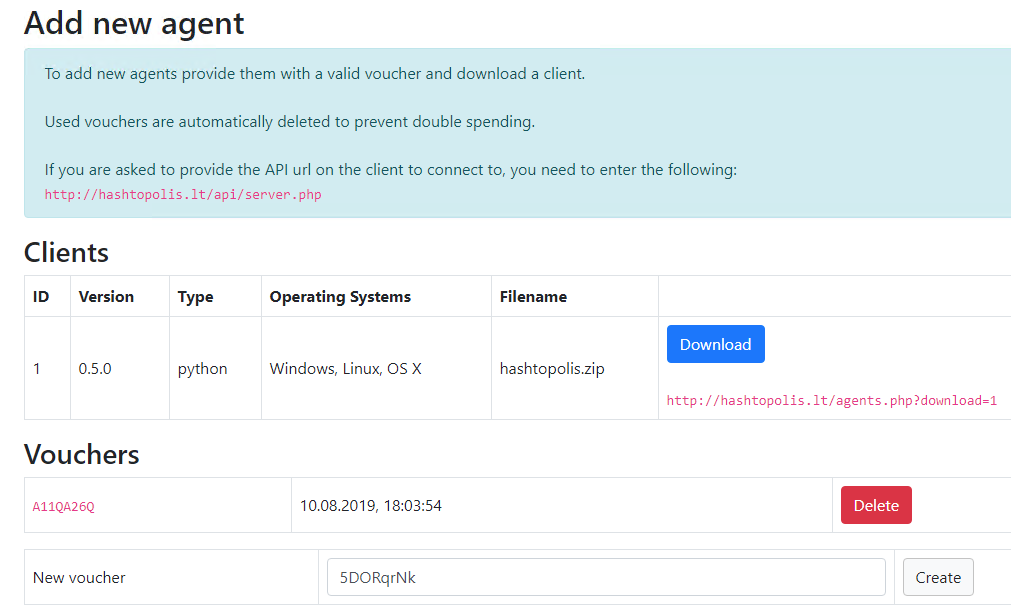
\includegraphics[width=\linewidth]{Immagini/8/hashtopolis_new_agent.png}
    \caption{Hashtopolis aggiunta di nuovi aggenti}
\end{figure}

Successivamente dobbiamo caricare nella piattaforma il file su cui eseguire l'attacco, andando a specificare il tipo di criptazione applicata su quei dati ed eventuali parametri passati.

\begin{figure}[ht]
    \centering
    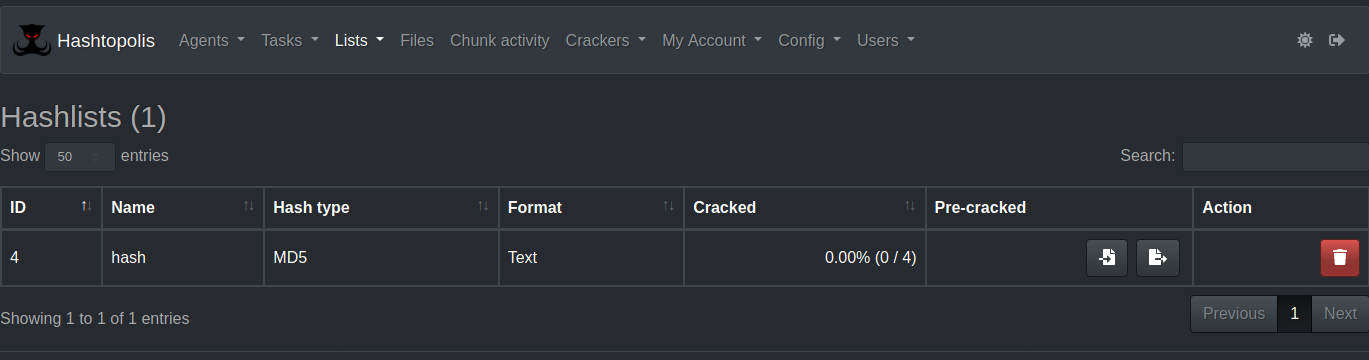
\includegraphics[width=\linewidth]{Immagini/8/hashtopolis_2.png}
    \caption{Hashtopolis aggiunta lista hash da attaccare}
\end{figure}

Hashtopolis ci peremtte di eseguire diversi tipi di attacco, per esempio possiamo eseguire attacchi Ruled based o Dictionary Attack, ma per eseguire questi tipi di attacchi, dobbiamo passare dei file di "configurazione", in questo caso noi per eseguire un Dictionary Attack, gli passiamo il dizionario rockyou, uno dei dizionari più utilizzati per eseguire questo tipo di operazione.

\begin{figure}[ht]
    \centering
    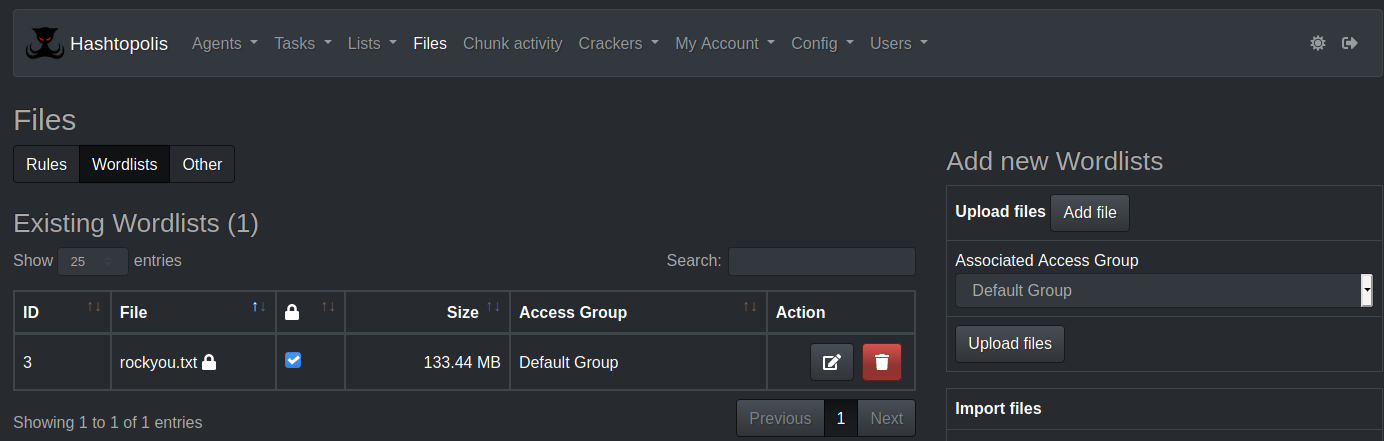
\includegraphics[width=\linewidth]{Immagini/8/hashtopolis_3.png}
    \caption{Hashtopolis aggiunta dizionario}
\end{figure}

Una volta configurati i file di cui si ha bisogno per eseguire l'attacco, si passa alla creazione della task, qui andremo ad associare :
\begin{itemize}
    \item un nome
    \item una lista di hash su cui eseguire il crack
    \item il dizionario/file delle regole
    \item priorità dell'attacco
    \item utilizzo di CPU, GPU o entrambe
    \item Gruppo che può eseguire l'attacco 
    \item ecc ecc 
\end{itemize}

\begin{figure}[ht]
    \centering
    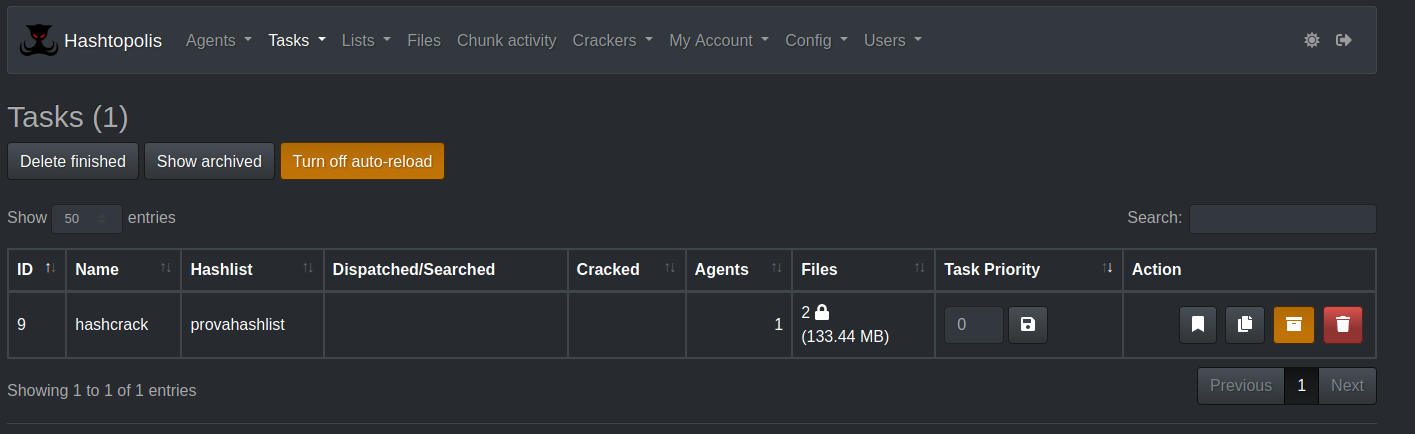
\includegraphics[width=\linewidth]{Immagini/8/hashtopolis_1.png}
    \caption{Hashtopolis creazione task}
\end{figure}

Dopo aver creato la task, ora possiamo andare ad associargli dei utenti, in modo da poter utilizzare la loro potenza di calcolo per eseguire l'attacco.

\begin{figure}[ht]
    \centering
    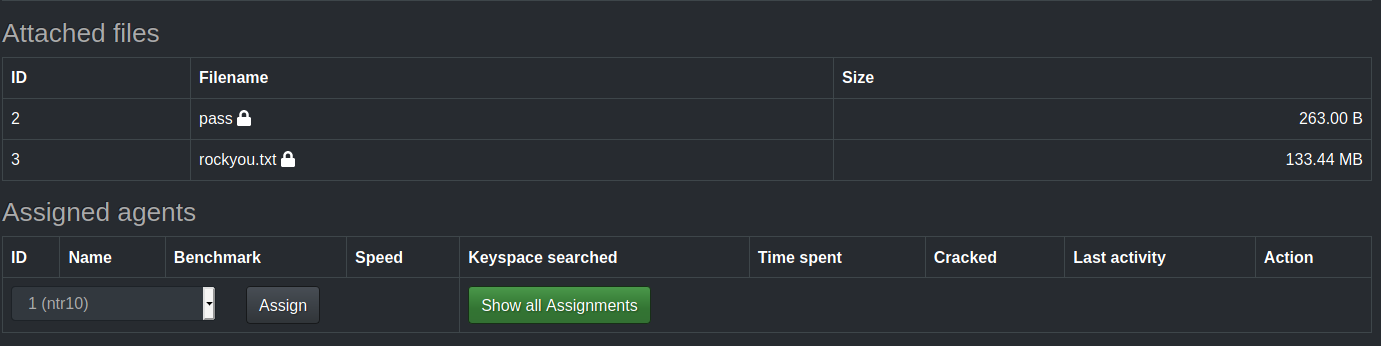
\includegraphics[width=\linewidth]{Immagini/8/hashtopolis_4.png}
    \caption{Hashtopolis aggiunta user a task}
\end{figure}

Una volta che uno user è stato associato ad una task, questo potrà eseguire lo script python, che lo colleghera al server e questo in automatico gli passerà i dati di cui ha bisogno per eseguire l'attacco e lui inizierà ad eseguire le varie operazioni.

\begin{figure}[ht]
    \centering
    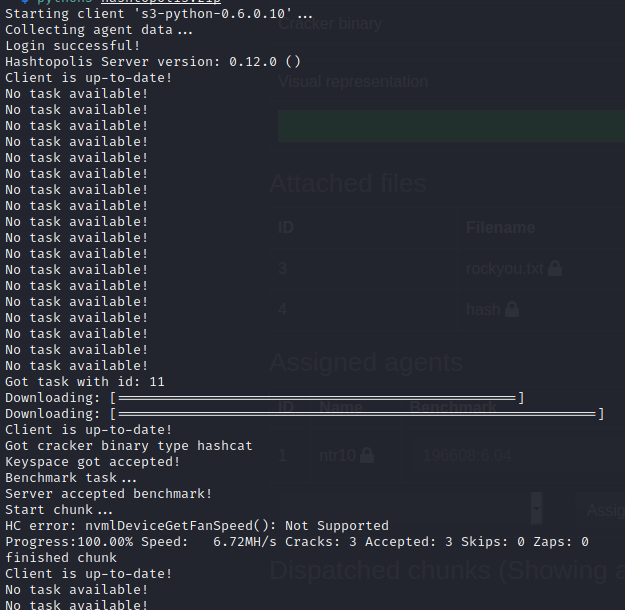
\includegraphics[width=\linewidth]{Immagini/8/hashtopolis_8.png}
    \caption{Hashtopolis client script}
\end{figure}

Dopo che l'utente avrà completato l'operazione, possiamo vedere nel sito di hashtopolis tutti i dati inerenti al crack, in modo da visualizzare quanti hash rimangono e quali sono stati risolti e quali ancora devono essere controllati.

\begin{figure}[ht]
    \centering
    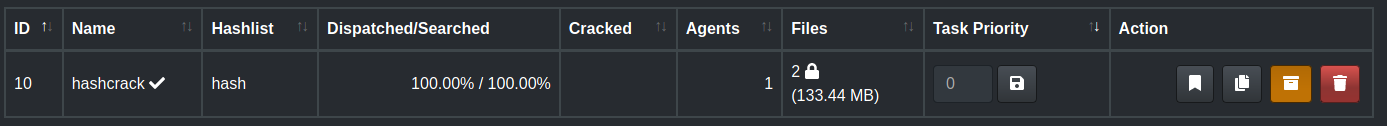
\includegraphics[width=\linewidth]{Immagini/8/hashtopolis_6.png}
    \caption{Hashtopolis task conclusa}
\end{figure}

All'interno di ogni task, possiamo vedere la suddivisione del lavoro tra i vari user che sono stati aggiunti alla task, qui possiamo vedere quanti hash hanno risolto e il tempo di esecuzione.
\newpage
\begin{figure}[ht]
    \centering
    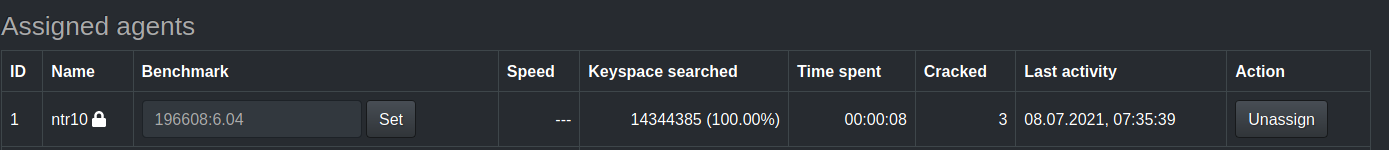
\includegraphics[width=\linewidth]{Immagini/8/hashtopolis_9.png}
    \caption{Hashtopolis suddivisione lavoro task per agent}
\end{figure}

Infine, una volta completata l'operazione, possiamo andare nella sezione hashlist, per visualizzare le password scoperte e quelle che ancora non sono state risolte.

\begin{figure}[ht]
    \centering
    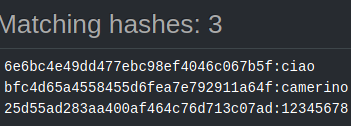
\includegraphics[width=\linewidth]{Immagini/8/hashtopolis_10.png}
    \caption{Hashtopolis password estratte}
\end{figure}

\label{chap:conc}
\chapter{Conclusioni}

Dopo aver studiato il funzionamento delle varie tecniche applicabili per eseguire un Brute Force, possiamo dire che alla stessa velocità con cui aumentano l'affidabilità dei algoritmi di criptazione delle nostre password, vengono trovati nuovi modi per decifrarli.

Come abbiamo potute vedere, le tecniche e i strumenti per eseguire questo tipo di operazioni, permettono di sfruttare diversi approcci (anche uniti tra di loro) e la potenza computazionale completa di un dispositivo, sia CPU che GPU, inoltre abbiamo potuto vedere anche tecniche che permettono di unire le potenze di calcolo di dispositivi diversi.

\section{Sviluppi futuri}

Uno dei problemi più grandi per chi attacca gli hash, è quello di incontrare algoritmi di criptazione troppo, complessi, ci sono alcuni algoritmi come : AES-256 e RSA, che per essere decriptati, richiedono una potenza di calcolo elevatissima, quasi infinitesimale, ma con l'avvenire delle nuove tecnologie e con il futuro avvento dei computer quantisci, anche questi algoritmi, potrebbere diventare obsoleti.

Il più grande problema nell'eseguire un Brute Force, è quello di avere la potenza di calcolo adeguata. Quindi i prossimi passi per gli attaccanti è quello o di trovare nuovi approcci per le esecuzione del Brute Force o quello di attendere l'arrivo di dispositivi con la potenza di calcolo necessaria.

\section{Problematiche}

Le varie tecniche e strumenti che abbiamo visto, anche se efficaci, hanno alcune problematiche, ecco alcuni esempi :

\begin{itemize}
    \item \textbf{Dictionary Attack} -> Le password non è contenuta nel dizionario, l'attacco non andrà a buon fine.
    \item \textbf{Mask Attack} -> bisogna conoscere la maschera da applicare
    \item \textbf{Rainbow Table } -> I file delle Rainbow Table, sono file di grandi dimensioni, viene richiesto un enorme spazio di archiviazione
    \item \textbf{Wi-Fi Brute Force} -> Bisogna essere in possesso di una scheda di rete che abbia la monitor mode
    \item \textbf{Hashtoplis } -> Utilizzando Mysql, le query a volte molto pesanti, possono risultare molto lente su database.
\end{itemize}

\section{Sistemi di difesa}

La miglior protezione è una buona password, che dobbiamo imparare a considerare importante al pari delle chiavi di casa. La maggior parte delle persone, invece, ne sottovaluta la rilevanza e per comodità sceglie combinazioni facili. Basti pensare che nel 2016 la password più utilizzata è stata “123456”, mentre il secondo posto è andato alla parola “password”, e il terzo al codice “12345678”. Un altro errore fatto molto spesso è quello di usare la stessa parola ripetuta al contrario. Una leggerezza che il cybercrime conosce molto bene: infatti, in Rete esistono decine di programmi gratuiti che sfruttano gli schemi comuni, permettendo di decifrare password poco complesse.

Una buona pratica per mettere a punto una password sicura è ideare parole chiave che utilizzino una combinazione di lettere maiuscole, minuscole, numeri e caratteri speciali. La si può ottenere, senza per forza rinunciare alla memorabilità. Un esempio sono gli acronimi di una frase semplice e rappresentativa come:

\medskip

Io mi chiamo Nico e ho 1 fratello  -->  ImcNeh1F

\medskip

Usa un gestore di password. L'installazione di un gestore di password automatizza la creazione e il monitoraggio delle informazioni di accesso online. Questi ti consentono di accedere a tutti i tuoi account accedendo prima al gestore di password. Puoi quindi creare password estremamente lunghe e complesse per tutti i siti che visiti, archiviarle in modo sicuro e devi solo ricordare l'unica password principale.

Usa password univoche per ogni sito che utilizzi. Per evitare di essere vittima del riempimento delle credenziali, non dovresti mai riutilizzare una password. Se vuoi aumentare la tua sicurezza, usa anche un nome utente diverso per ogni sito. Puoi evitare che altri account vengano compromessi se uno dei tuoi viene violato.
\begin{figure}[ht]
    \centering
    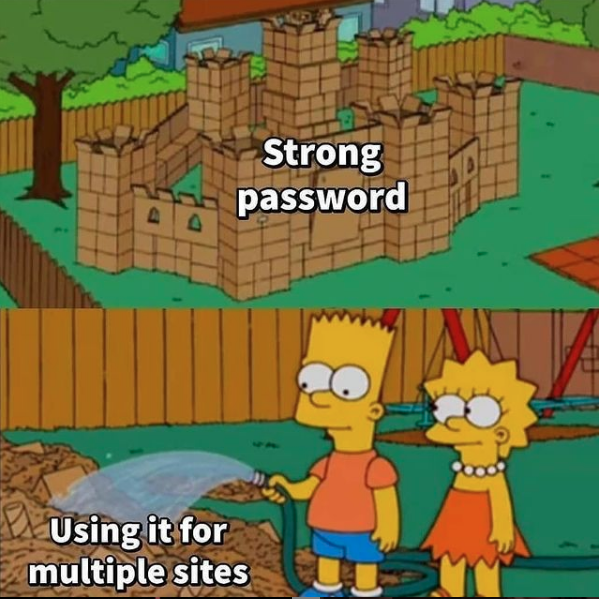
\includegraphics[width=90mm]{Immagini/9/simpson.png}
\end{figure}

\newpage

\subsection{10 Comandamenti del Hash Cracking}

\begin{enumerate}

    \item Conoscerai i tipi di hash e la loro origine/funzione
    \item Conoscerai i punti di forza e di debolezza dei software di cracking
    \item Studierai e applicherai tecniche di analisi delle password
    \item Devi essere esperto nei metodi di estrazione dell'hash
    \item Creerai dizionari personalizzati/mirati
    \item Conoscerai le capacità delle tue piattaforme di cracking
    \item Comprenderai la psicologia/comportamento umano di base
    \item Creerai maschere, regole personalizzate
    \item Sperimenterai continuamente nuove tecniche
    \item Sosterrai i tuoi compagni di cracking membri della comunità

\end{enumerate}


\lstlistoflistings
\listoffigures
\listoftables

\appendix
%\input{schema_elettrico}
%\input{Appendix1}
%\input{Appendix2}

\printbibliography

\printindex

\chapter*{Ringraziamenti}

Ringrazio...

\end{document}